\chapter{Introduction}\label{intro}

	Say something profound here.
	
	Structure of this thesis:
	
		Gravitational waves and their detection
	
		The LIGO instrument and Noise + Squeezed States of Light
	
		Introduction to Wavefront Sensing
	
		Experimental Mode Matching at Syracuse
	
		Mode matching at LIGO Hanford
	
		Future Works

	\section{Gravitational Waves}\label{gravitational waves}
	In 1915, Albert Einstein published his theory of general relativity \cite{einstein}, which contains the most complete description of gravity to date. The seminal equation in this theory, called the Einstein Field Equation is
	
	\begin{equation} \label{einstein}
	G_{\mu \nu} = 8 \pi T_{\mu \nu}
	\end{equation}
	
	which is a set of 10 coupled second-order differential equations that are nonlinear and fully describes the interaction between space-time and mass-energy. Equation \ref{einstein} is difficult to solve except in situations where specific approximations allow a user to find exact solutions such as spherical symmetry \cite{carroll_2003} \cite{schutz_2009}. In areas where the curvature is close to flat,  the weak field approximation can be applied and the metric is described as	
	
	\begin{equation} \label{weak}
	g_{\mu \nu}  \approxeq \eta_{\mu \nu} + h_{\mu \nu}
	\end{equation}
	
	where $\eta_{\mu \nu}$ is the metric of flat space time and $|h_{\mu \nu}| \ll 1$ is the perturbation due to a gravitational field.
	
	By plugging in equation \ref{weak} into \ref{einstein} and using empty space we obtain the familiar wave equation
	
	\begin{equation} \label{wave}
	\Big(\nabla^2 - \frac{1}{c^2} \pdv[2]{t} \Big) h_{\mu \nu}  = 0
	\end{equation}

	which has a plane-wave solution of the form $h_{\mu \nu} = A_{\mu \nu} e^{ik_{\nu} x^{\nu}}$. 
	
	Using the gauge constraint $h^{\mu \nu}_{,\nu} = 0$, it follows that $A_{\mu \nu} k^{\mu} = 0$ which means that the gravitational wave amplitude is orthogonal to the propagation vector.
	
	Further imposing transverse-traceless gauge and assuming that the wave is traveling in the $x^3$ direction, it can be shown that the complex amplitude has physical significance expressed in the matrix
	
	\begin{equation} \label{gwamp}
	A_{\mu \nu} = 
	\begin{pmatrix}
			0 &    0   &  0      & 0 
		 \\ 0 & A_{xx} &  A_{yx} & 0
		 \\ 0 & A_{xy} & -A_{xx} & 0
		 \\ 0 &    0   &  0      & 0
	\end{pmatrix}
	\end{equation}

	Oftentimes, the four non-zero components of equation \ref{gwamp} can be categorized into two distinct polarizations called plus and cross such that $h_{+} = A_{xx} = -A_{yy}$ and $h_{\cross} = A_{xy} = A_{yx}$ .
 
	It is natural to attempt to understand the physical interpretation of equation \ref{gwamp} as an affect on the position of a free floating particle. Consider the four-velocity, $U^{\alpha}$, in the transverse traceless gauge where the coordinate itself is attached the particles and incorporates any small wiggles that would shake the coordinates.  Of course, any free particles will follow the geodesic equation
	\begin{equation}\label{geodesic}
	\nabla U^{\alpha} = \frac{\text{d}}{\text{d} \tau} U^{\alpha} + \Gamma^{\alpha}_{\mu \nu} U^{\mu} U^{\nu} = 0
	\end{equation}	
	where $\Gamma^{\alpha}_{\mu \nu} = \frac{1}{2} g^{\gamma \alpha}(g_{\gamma \mu, \nu} + g_{\gamma \nu,\mu} - g_{\mu \nu, \gamma} )$ are the famous Christoffel symbols.
	By evaluating the first term of the acceleration in equation \ref{geodesic},
	\begin{equation}\label{accel}
	\bigg(\frac{\text{d}U^{\alpha}}{\text{d}\tau}\bigg)_0 = -\Gamma^{\alpha}_{00} 
	\\ = \frac{1}{2} \eta_{\mu \nu} (h_{\beta 0, 0} + h_{0 \beta, 0} + h_{0 0, \beta} )
	\end{equation}
	
	\begin{figure}[h]
		\centering
		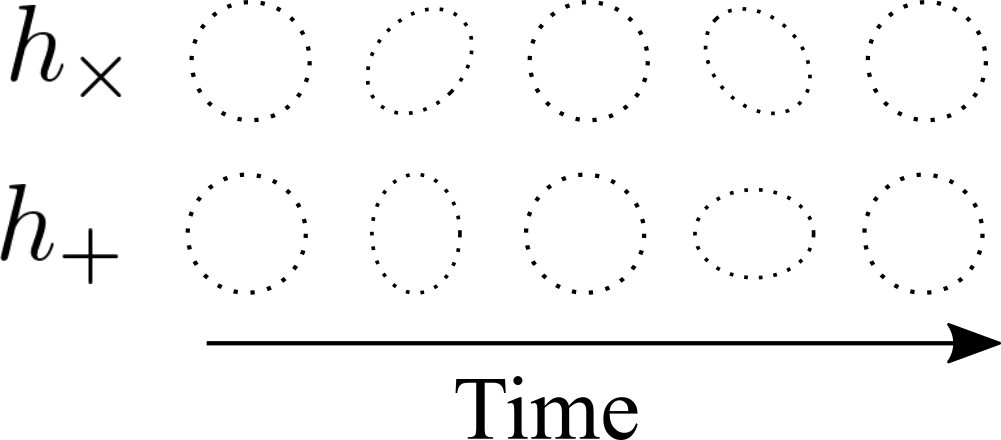
\includegraphics[width=.5 \textwidth]{../Figures/GW_Particles.png}
		\caption{A ring of free floating particles will be stretched and squeezed if a gravitational wave passes through them.  The polarization will affect the particles in a similar way but rotated 45 degrees.}
		\label{fig:gwparticles}
	\end{figure}
	
	However, comparing equation \ref{gwamp} and equation \ref{accel}, it is clear that if the particle is initially at rest, then a moment later it is still at rest! The term "at rest" is actually used liberally here since the coordinate system varies along with the gravitational wave. 
	
	Alternatively, one can ask if a gravitational wave passed by a pair of particles separated by length $L$, what would be the effect on the distance between two points?  The proper distance is defined as

	\begin{equation}\label{propdist}
	\delta l
	= \int{g_{\mu \nu} dx^{\mu} dx^{\nu}} \\
	= \int_{0}^{L}{g_{xx} {d}x}\\
	\approx |g_{xx}(x=0)|^{1/2}\\
	\approx [ 1 + \frac{1}{2} h_{xx}(x=0)] L
	\end{equation} 
	
	which shows us two very important points about the nature of gravitational waves.  Firstly, the effect is very small since the length variation, $h_{xx}$, is a small perturbation on flat space-time.  Secondly, the effect is proportional to the initial separation between the particles. This means a detector which is large will have a better chance to measure these small effects, an important point that drove the design of the Laser Interferometer Gravitational-Wave Interferometer (LIGO).
	
	\subsection{Measuring Gravitational Waves with Light}\label{measuringGWs}
	Even with the theoretical formulation of gravitational waves resolved by the 1970s \cite{PiraniPhysicalSignificance}, the possibility of detecting gravitational waves by ground-based instruments was still a controversial topic among scientists in the field \cite{CollinsGravity}.  During the famous Chapel Hill Conference in 1957 which included some of the great minds of the era such as Wheeler, Schwinger, and Feynman, the experimental search for gravitational waves began to take hold.  One thought experiment that was proposed by Feynmann \cite{SmootBrief} where he considered a bead sliding on a string with some friction as a gravitational wave passes by.  As the beads slide back and forth due to the wave described by equation \ref{propdist}, there will be some heat dissipated which means the gravitational wave must carry some energy.
	
	There is still the issue of an incredible amount of accuracy required to measure the strain from even the most dense astrophysical objects. The earliest attempts at detecting these small signals were famously done by Joseph Weber using large resonant bars and piezoelectric transducers to extract the energy from gravitational waves at the resonant frequencies of the bars. Picture of bar detectors at LHO.  However, these bars are limited by thermal noise and can only detect GWs in very narrow frequency bands. 
	
	Interferometers are devices that measure small displacements by using a laser that is split by a partially transmitting mirror (or beamsplitter), which allows 50$\%$ of the light to get reflected and 50$\%$ to be transmitted.  Each of the beams travel down the arms and reflect off of mirrors and return to the beamsplitter.  Upon reaching the optic, the two beams recombine and by the principle of superposition  the electromagnetic waves will add linearly at the output port (or antisymmetric port). Figure[].  The laser beams will gather phase as they propagate down each individual arm, and when recombining, the intensity of the light will be proportional to the phase differences between each beam.  This will correspond to a differential length that is described by
	
	\begin{equation}
	L_{-} = l_{x} - l_{y}
	\end{equation}
	
	As shown in equation \ref{propdist}, the effect of gravitational waves on the proper length between two free falling objects is proportional to the initial separation.  From figure[GWparticles], it is intuitively clear that interferometry would be an ideal technique to detect signals from a gravitational wave.  However, one can explicitly derive a ground-based interferometer's response to a GW from an astrophysical object.
	
	Consider a gravitational wave source arbitrarily located in the sky with respect to an interferometer on Earth. By denoting the interferometer's Cartesian coordinates as $\{\hat{x},\hat{y},\hat{z}\}$ with x and y located along the arms respectively such that the z-axis points directly towards the zenith (i.e. a right-handed system.).  Using the well known Euler angles, a relation from the detector frame to the source frame with coordinates $\{\hat{x}',\hat{y}',\hat{z}'\}$ can be seen in Figure[Euler]. 
	
	If a gravitational wave at the source has emitted GWs with plus and cross polarizations as denoted by equation \ref{gwamp}, then the detector time series can be regarded as \cite{S6sensitivity} \cite{Finn:1995}
	\begin{equation}
	h(t) = F_{+}(\theta,\phi,\psi) \, h_{+}(t) + F_{\times}(\theta,\phi,\psi) \, h_{\cross}(t)
	\end{equation}
	where $F_{+}(\theta,\phi,\psi)$ and $F_{\cross}(\theta,\phi,\psi$ are the antenna pattern functions that project the gravitational wave amplitudes onto the detector frame.
	
	\begin{equation}\label{Fplus}
	F_{+}(\theta,\phi,\psi) = -\frac{1}{2}[1+\text{cos}^2(\theta)] \text{cos}(2\phi) \text{cos}(2\psi) - \text{cos}(\theta) \text{sin}(2\phi) \text{sin}(2\psi)
	\end{equation}
	\begin{equation}\label{Fcross}
	F_{\cross}(\theta,\phi,\psi) = + \frac{1}{2}[1+\text{cos}^2(\theta)] \text{sin}(2\phi) \text{cos}(2\psi) - \text{cos}(\theta) \text{sin}(2\phi) \text{sin}(2\psi)
	\end{equation}
	
	If the gravitational wave is located directly above the interferometer such that $\theta = 0$ and setting $\psi=0$, then the magnitude of the antenna pattern is equal to unity.  Furthermore, by rotating about the $\phi$ angle such that the detector arms align with the plus polarization, the null geodesic equation (ie the path of a photon) in the interferometer frame becomes 
	
	\begin{equation}
	ds^2 = g_{\mu\nu}dx^{\mu} dx^{\nu} = -dt^2 + [1+h_{+}]  dx^2 + [1-h_{+}]  dy^2 + dz^2 = 0
	\end{equation}
	
	Now, if the photon is traveling along the x-arm, this means that $dy^2 = dz^2 = 0$ and the metric equation transforms to
	
	\begin{equation}
	\frac{dt}{dx} = \sqrt{ 1+h_{+} } \approx 1+\frac{1}{2} h_{+} 
	\end{equation}
	
	The amount of time required for the photon to reach the x-end mirror (starting at $t=0$) is equal to
	
	\begin{equation}\label{pathlength}
	t_1 = \int_{0}^{L_{x}} [1+\frac{1}{2}  h_{+}(x) ] \text{d}x
	\end{equation}
	
	where $L_x$ is the total length of the x-arm.  Upon returning to the beamsplitter, the photon's total time of flight for the x and y arms are, respectively,
	
	\begin{equation}
	t_2 = 2 L_x + \frac{1}{2} \int_{0}^{L_x} \bigg[  h_{+}(x) +  h_{+}(x + L_x)  \bigg] \text{d}x
	\end{equation}
	\begin{equation}
	t'_{2}= 2 L_y - \frac{1}{2} \int_{0}^{L_y} \bigg[  h_{+}(y) +  h_{+}(y + L_y)  \bigg] \text{d}y
	\end{equation}
	
	If the gravitational wave period is much longer than the time of flight, then $h_{+}$ does not change much during the measurement, which means $h_{+}(\eta_i) \approx h_{+}(\eta_i + L_{\eta_i}) \approx constant$.  By subtracting the flight times of the photons for each arm and setting $L = L_x = L_y$, the difference is proportional to the gravitational wave perturbation multiplied by the sum of arm lengths (with a factor of $c$ to get the units right),
	
	\begin{equation}
	\Delta t = t_2 - t'_{2} = \frac{2L}{c} h_{+}
	\end{equation}
	
	By recasting the expression for time of flight in terms of the phase picked up laser light as it travels through space, the differential phase shift is
	\begin{equation}\label{diffphase}
	\Delta \Phi = \Phi(t_{2}) - \Phi(t'_{2}) = \frac{4 \pi}{\lambda} \, h_{+} \, L
	\end{equation}
	
	The equation above is simple, however, it only works for gravitational wave signals that are not frequency dependent and it assumes that the path length can be arbitrarily long. Both points are actually not true \cite{Saulson} but we can alleviate these discrepancies by considering a gravitational wave signal of the form $h(t) = h_0 \text{exp} (i 2 \pi f_{GW} t)$  and repeating the calculation between equations \ref{pathlength} and \ref{diffphase}:
	
	\begin{equation}\label{gwsinc}
	\Delta \Phi (t) = h(t) \; \tau_{RT} \; \frac{2 \pi c}{\lambda} \; \text{sinc}(f_{GW} \tau_{RT}) e^{i \pi f_{GW} \tau_{RT}}
	\end{equation}
	
	where $\tau_{RT} = 2L/c$.  The response for a detector whose arm lengths are blank km have null points at the around blank Hz which means the instrument cannot be arbitrarily long, however, this point is not concerning because it is too expensive and difficult to make a terrestrial detector of this size.
	
	How to practically measure $\Delta \Phi$ with an interferometer is explained in section \ref{LIGOInstrument}.

	\subsection{Detection of Gravitational Waves}\label{detectgw}
	The purpose of LIGO is to observe gravitational waves emanating from astrophysical objects \cite{NSFproposal}, so it is natural to wonder how well a single detector can probe the universe.  It is worthwhile to explicitly derive the inspiral horizon distance, which is how far a single detector can see a source comprised two equal mass compact objects optimally oriented in the sky relative to the detector.  Signal-to-noise (SNR) is the level of interesting signals compared to the background noise, which can be expressed as
	\begin{equation}\label{SNR}
	\rho = 2 \int_{-\infty}^{\infty} \frac{ \tilde{s}(f) \tilde{s}^*(f) }{S_n(f)}
	\end{equation}
	
	where ${S_n(f)}$ is the one-sided average power spectral density of the detector noise and $\tilde{s}(f)$ is the Fourier transform of the detectors' response to a gravitational-wave signal.
	
	Consider two dense objects with mass $m_1$ and $m_2$ rotating around each other, separated by a distance $R$ such that quadrupole equation still holds (i.e. flat space-time with small perturbations). The detector response, in units of strain, to the gravitational waves emitted by this source is \cite{Finn:1995},
	
	\begin{equation}\label{inspiralsignal}
	s(t) = \frac{\mathcal{M}}{d_L} \Theta(\theta,\phi,\psi,i) [\pi f(t) \mathcal{M}]^{2/3} \cos[\Phi(t) + constant]
	\end{equation}
	where 

	\begin{subequations}
		\begin{equation}\label{chirp}
	\mathcal{M} \&= (1+z) \frac{(m_1 m_2)^{3/5}}{(m_1 + m_2)^{1/5}}
		\end{equation}
		\begin{equation}\label{orient}
	\Theta(\theta,\phi,\psi,i) \&= 2 \sqrt{	[F_{+}(\theta,\phi,\psi) (1+\cos^2(i)) ]^2 + [2 F_{\cross} \cos(i)]^2 }
		\end{equation}
	\end{subequations}

	By convention, $\mathcal{M}$ called the chirp mass and $d_L$ is the luminosity distance. The orientation response, $\Theta(\theta,\phi,\psi,i)$, is a function that depends entirely on the detector orientation relative to the angular momentum vector of the binary [Figure of a binary spiraling and a detector on earth]
	
	
	where $F_{+}$ and $F_{\cross}$ are from equation \ref{Fplus} and \ref{Fcross}.
	
	As the binary loses energy to gravitational waves, the orbit will shrink as a function of time, in turn, the orbital frequency will increase
	
	\begin{equation}
	f(t) = \frac{1}{\pi \mathcal{M}} \bigg[\frac{5}{256} \frac{\mathcal{M}}{T-t}\bigg]^{3/8} 
	\end{equation}
	
	By defining the binary phase as $f(t) = \frac{1}{2\pi} \frac{\partial \mathbf{\Phi} }{\partial t}$, it is easy to recognize that the phase also evolves with time.
	\begin{equation}
	\Phi(t) = 2\pi \int_{T}^{t} f(t) dt = -2 \bigg( \frac{T-t}{5\mathcal{M}}\bigg)^{5/8}
	\end{equation}
	
	What this means is that the gravitational wave signal from the binary will increase in amplitude and frequency as a function of time up until the coalescence time, $T$.


	There is actually a subtle difference between the coalescence time and the moment when adiabatic approximations fail which allows usage of the quadrupole formulation. 

	Plugging equation \ref{inspiralsignal} into \ref{SNR},
	\begin{equation}
	\rho = 8 \Theta(\theta,\phi,\psi,i) \frac{r_0}{d_L} \bigg(\frac{\mathcal{M}}{1.2 \textup{M}_\odot}\bigg)^{5/6} \zeta(f_{max})
	\end{equation}
	
	There are two important functions in the equation above that reflect the detector's performance in sensing gravitational radiation from a binary inspiral, $r_0$ and $\zeta(f_{max})$.
	
	The characteristic distance, $r_0$ is how far the detector can see for a fixed binary's mass distribution,
	
	\begin{equation}\label{char_r0}
	r_0^2 = \frac{5}{192\pi^{4/3}} \bigg(\frac{3\textup{M}_\odot}{20}\bigg)^{5/3}   \int_{0}^{\infty} \frac{1}{S_n(f)} \frac{\text{d} f}{f^{7/3}}
	\end{equation}

	Due to the integrand's dependence on $f^{-7/3}$, lower frequency improvements in the detector's noise spectrum will contribute more to the distance.
	
	\begin{equation}\label{zeta}
	\zeta(f_{max}) = \frac{\int_{0}^{2f_{max}} \frac{1}{S_n(f)} \frac{\text{d} f}{f^{7/3}}}{\int_{0}^{\infty} \frac{1}{S_n(f)} \frac{\text{d} f}{f^{7/3}}}
	\end{equation}
	
	The sensitivity can be different for various mass distributions; $\zeta(f_{max})$ is a normalized function that describes how well the detector's bandwidth overlaps the binary's frequency evolution.  If $f_{max}$ is higher that the minimal sensitivity frequency for the detector, then there is good overlap and  $\zeta(f_{max})\approx 1$.  However, if the masses are sufficiently large, $f_{max}$ will be lower because coalescence occurs before the objects reach a higher frequency regime and this will result in  $\zeta(f_{max})\approx 0$.
	
	The process of two objects coalescing starts at lower frequencies and terminate at some $f_{max}$ that depends on when the objects reach their inner-most stable circular orbit, $f_{ISCO}$.   If $m_1=m_2$, then the maximum frequency is[]
	
	\begin{equation}
	\begin{aligned}
	f_{max}	=&  \frac{f_{ISCO}}{1+z} \\
			=&	\frac{99 \text{Hz}}{1+z} \, \frac{20 \textup{M}_\odot}{M}
	\end{aligned}
	\end{equation}
	where $M=m_1+m_2$.

	By plugging a few mass distributions and an estimate of the sensitivity [GWINC], it is possible to study the range of a single detector.  For example, a 1.4-1.4$\textup{M}_\odot$ binary that has optimal orientation with respect to the detector has horizon distance equal to...
	
	Horizon distance and range, advanced LIGO projected
	
	[Finn, Duncan Thesis]
	\cite{Saulson}
	
	\section{The LIGO Instrument}\label{LIGOInstrument}
	In its simplest form, the LIGO instrument is an incredibly large Michaelson interferometer.  
	If we imagine the output as a measure of differential arm length, it becomes a natural way of detecting gravitational waves. 
	However, to make a practical gravitational-wave observatory, the complexity will have to be extended beyond what Michelson and Morley used.  
	The next sections will explore the various upgrades to the instrument configuration that improve the sensitivity of LIGO.
	
		\subsection{Simple Michaelson}\label{michelson}
		As shown in Figure [michelsonifo], the interferometer begins with a laser which is incident on a partially-reflecting and partially-transmitting beamsplitter that sends half of the laser light down each arm.  The individual beams gather phase as they propagate down the arms and then reflect off of two end mirrors and eventually recombine at the same beamsplitter.  Whether the light constructively or destructively interferes will depend on their relative accumulated phase from propagating down each arm. A photodetector is placed at the output and measures the total power which converts the total amount of light into an electronic signal.
		
		In Section \ref{measuringGWs}, it was shown that the differential time of flight between photons traveling down the individual arms carry gravitational wave information.  
		The difference in flight times, $\Delta t$, can be converted into how much phase, $\Delta \phi$, is accumulated by the photons as they propagate through space.  
		
		But the question remains, how does an interferometer explcitly measure $\Delta \phi$?
		
		If the input electric field of the interferometer is $E_0$, the beamsplitter will transmit $iE_0 /\sqrt{2}$ down the x-arm and reflect $E_0 /\sqrt{2}$ towards the y-arm.  By setting the beamsplitter to be the origin, the two plane waves traveling down their respective arms will have gathered a phase $\phi_i$. Then, upon reflecting off the end mirrors and returning to the beamsplitter where the x-arm reflects and the y-arm transmits to the output port. Each of the electric fields can be described by these equations
			\begin{equation}
			\begin{aligned}
				E_{x} 	&=	\frac{i E_0}{2} e^{2i\phi_{x}}	
			\\	E_{y} 	&=	\frac{i E_0}{2} e^{2i\phi_{y}}
			\end{aligned}
			\end{equation}
		Since the electromagnetic waves are linear, the resultant sum of waves at the antisymmetric port will be $E_{out} = E_x + E_y$. The photodiode at the output (or antisymmetric) port detects the integrated power which is related to the total electric field by
			\begin{equation}
			\begin{aligned}\label{asy_power}
				P_{AS}	&= \int_{\text{Area}} I \;				\text{d}A 
			\\			&= \int_{\text{Area}} \vert E_x + E_y \vert^2 \;	\text{d}A 
			\\			&= P_{in} \; \cos^2(\Delta \phi)
			\end{aligned}
			\end{equation}	
		where $\Delta \phi = \phi_{x} - \phi_{y} = k_x L_x - k_y L_y$ and $P_{in} = \int_{\text{Area}}	 \vert E_0\vert^2 \text{d}A$ is the input power. By using equation \ref{diffphase} and the common (or average) arm length $L_{+} = \frac{L_x + L_y}{2}$, the power due to a differential phase shift is
			\begin{equation}
			P_{AS} \approx P_{in} \; (1-2 \Delta \phi) = P_{in} \; (1-2 k L_{+} h_{+})
			\end{equation}
		There is a large DC term that is dependent on the input power and generally, it is very difficult to measure small changes in a large signal. So the next obvious method would be to shift the arms such that the output port is operating on a dark fringe, normally this is called a null-point operation.  However, there are difficulties associated with this method as well.  
		Consider shifting the phase of equation \ref{asy_power} by $\pi/2$, which would result in
			\begin{equation}\label{null}
			P_{AS} \vert_{null} = P_{in} \; \text{sin}^2 (\Delta \phi) \approx P_{in} \; (k L_{+} h_{+})^2 
			\end{equation}
		This results in a second-order dependence on a gravitational-wave signal that is already approximated to be very small.  
		So a good solution to the issue of how to $read$ out a gravitational wave signal can be solved using radio frequency (RF) detection methods. Consider changing the interferometer input by adding an electro-optical modulator (EOM) to sinusoidally modulate the laser frequency and expanding to first order using the Bessel functions,
			\begin{equation}\label{modE}
			\begin{aligned}
			E_{in} 	&= E_{0} e^{i(wt + \beta \text{cos} (\Omega t))} \\
					&\approx E_0 e^{iwt} [J_0(\beta) + J_1(\beta) e^{i \Omega t} + J_1(\beta) e^{-i \Omega t}] \\
					&= E_{C,in} + E_{SB+,in} + E_{SB-,in}
			\end{aligned}
			\end{equation}
		where $\Omega$ and $\beta$ are the modulation frequency and depth, respectively. The first term is commonly called the carrier field whereas the second and third terms are referred to as the (upper or lower) sidebands.  Because there are multiple electric fields, it is useful to define an optical transfer function which transforms the interferometer's input fields to its output,
		\begin{equation}\label{opt_tf}
		E_{out} = E_{C} + E_{SB+} + E_{SB-} = 
		\begin{pmatrix}
			t_{C} 	&   
		\\ 	t_{SB+} &
		\\ 	t_{SB-} &
		\end{pmatrix}
		\begin{pmatrix}
		E_{C,in} &    E_{SB+,in}    &  E_{SB-,in}     
		\end{pmatrix}
		\end{equation}
		The carrier transfer function, $t_{C}$ has already been calculated by equations \ref{asy_power} - \ref{null} and the sideband transfer functions are not much different.
		\begin{equation}\label{sb_tf}
		t_{SB\pm} = r_{x,\pm}  e^{i\phi_{\pm,x}} - r_{y,\pm}  e^{i\phi_{\pm,y}}
		\end{equation}
		where $\phi_{\pm,i} = (k \pm k_{\Omega}) \, \ell_{i} = (\frac{w+\Omega}{c} ) \ell_{i}$. In the current example, the sidebands and carrier fields reflect off the end mirrors identically, however, this will not be true in general when dealing with resonators that are highly frequency dependent.  Plugging equation \ref{sb_tf} into \ref{opt_tf}, the output electric field becomes 
		\begin{equation}
		E_{out} = i e^{iwt} [ J_0(\beta) 	k \ell_{+}  h_{+}  \; + \; J_1(\beta) \sin( k \Delta \ell + k_{\Omega} \Delta \ell) (e^{i\Omega t}  + e^{-i\Omega t}) ]
		\end{equation}
		The frequency offset of the sidebands allow them to pick up phase differently than the carrier field. Thus, by choosing a static offset between the arm lengths such that the carrier signal is on a dark fringe, $k \Delta \ell = \pi/2$, but the sideband are slightly off the null point (Figure [\ref{fig:MichelsonHetero}]) and hence leak into the anti-symmetric port.  This technique is colloquially known as the Schnupp Asymmetry and the electric field reduces to
		\begin{equation}
		E_{out} = i e^{iwt} [ J_0(\beta) 	k \ell_{+}  h_{+}  \; + \; J_1(\beta) \sin(k_{\Omega} \Delta \ell) ( e^{i\Omega t} + e^{-i\Omega t}) ]
		\end{equation}
		
		\begin{figure}[h]
			\centering
			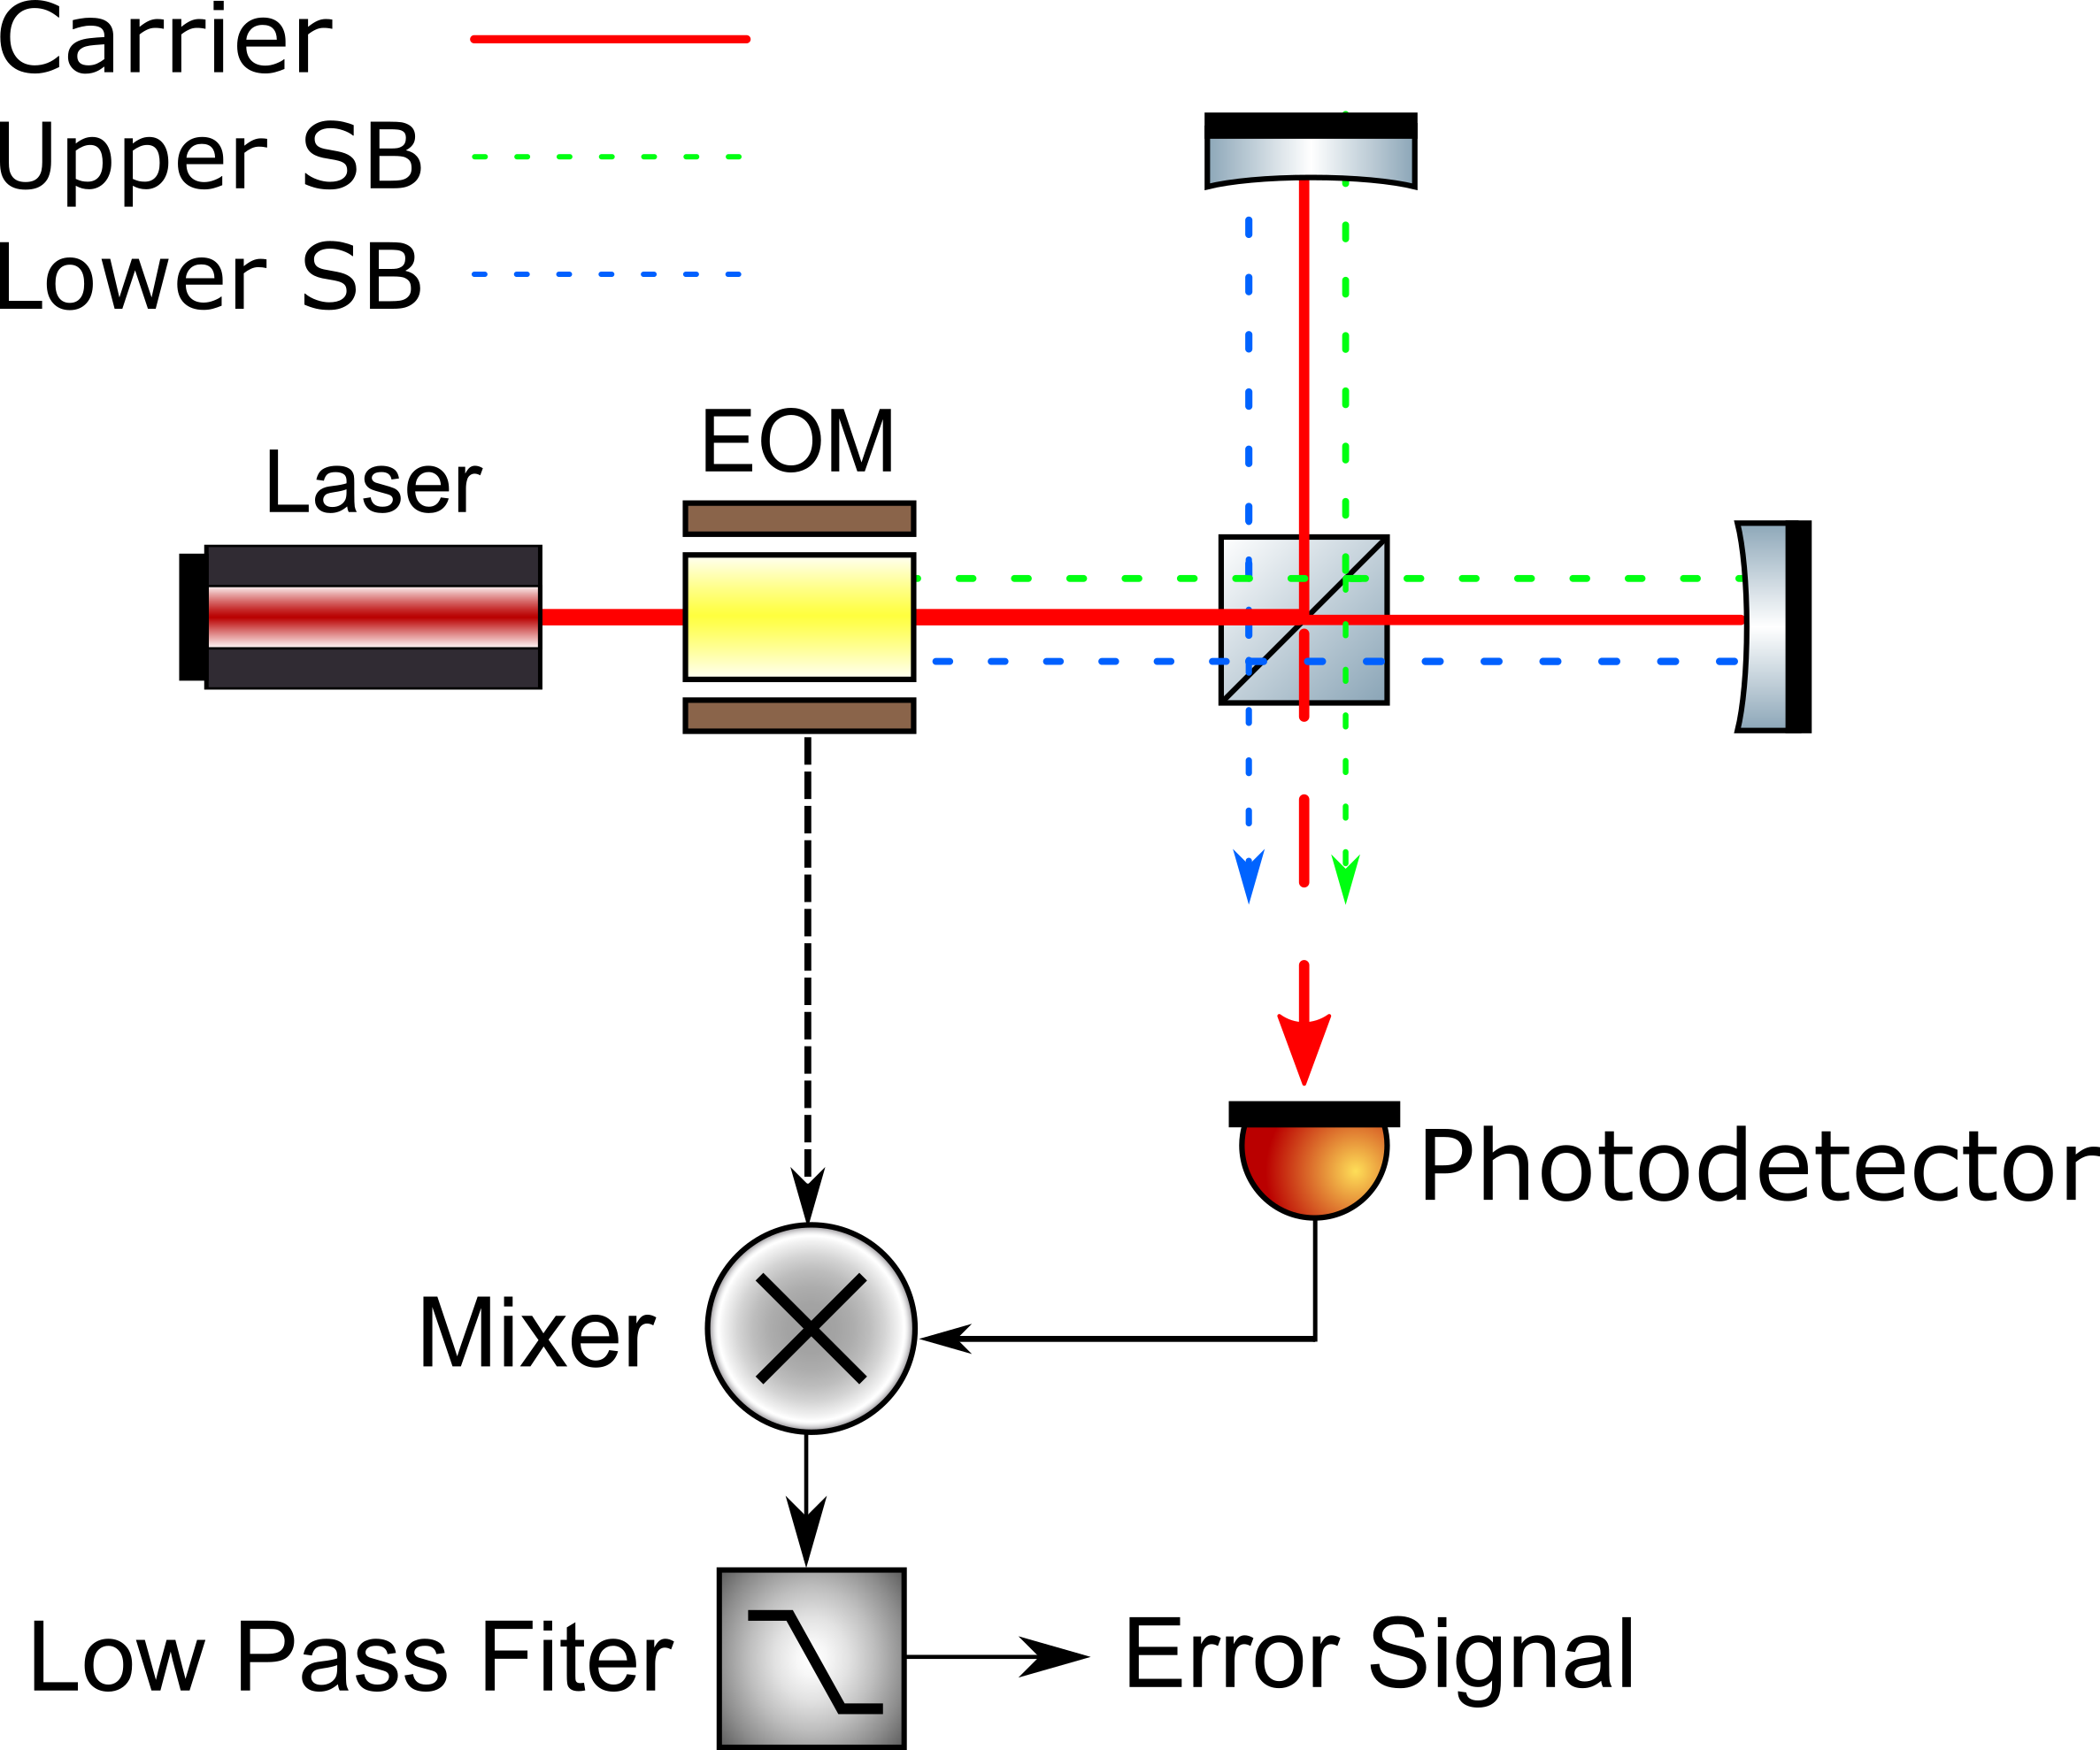
\includegraphics[width=.65 \textwidth]{../Figures/SimpleMichelsonHetero.png}
			\caption{Michelson with heterodyne detection scheme.}
			\label{fig:MichelsonHetero}
		\end{figure}
		
		
		
		Recall that the intensity is equal to the electric field squared,
		\begin{equation}\label{RFdet}
		\begin{aligned}
			I	= \vert E_{out} \vert^2  =	&\vert E_{C}\vert^2 + \vert E_{SB+}\vert^2 + \vert E_{SB-}\vert^2 \\
										  	& + 2 \mathbf{Re} \{ \; E_{SB+} E^*_{SB-} e^{2i\Omega t} \; \}\\
										  	& + 2 \mathbf{Re} \{ \; (E_{C} E^*_{SB-} +  E_{SB+} E^*_{C} ) e^{i\Omega t} \; \}
		\end{aligned}
		\end{equation}
		The last term is referred to as the $beat$ $note$ between the carrier signal and the sidebands.  It is possible to extract the term at the modulation frequency using a mixer which is an analog device that outputs the product of two inputs. Usually, the same oscillator that was used to modulate the input beam can be one of the mixer inputs, $\cos(\Omega t)$,  so that the demodulated signal is
		\begin{equation}
		\begin{aligned}
		I_{Demod} 	&\propto \big[ 4 \pi  J_0(\beta) J_1(\beta) \frac{\ell}{\lambda}  \sin(k_{\Omega} \Delta \ell)  \; h_{+}\big] \big[ \cos(\Omega t)  \sin(\Omega t + \phi_{Demod}) \big] \\
					&\propto \big[ 4 \pi  J_0(\beta) J_1(\beta) \frac{\ell}{\lambda}  \sin(k_{\Omega} \Delta \ell)  \; h_{+}\big] \big[ \sin(\phi_{Demod}) + \sin(2\Omega t + \phi_{Demod}) \big]
		\end{aligned}
		\end{equation}
		where $\phi_{Demod}$ is the phase that can be set by the user in order to account for extra phase shifts (ie. longer cables). After the mixer, there will be signals at DC, $\Omega$, $2\Omega$ and so on. However, the part that is linear in the gravitational wave amplitude will be at DC so a low-pass filter will allow the final signal to dominate:
		\begin{equation}
		S = 4 \pi  J_0(\beta) J_1(\beta) \frac{\ell}{\lambda}  \sin(k_{\Omega} \Delta \ell) \sin(\phi_{Demod}) \; h_{+}
		\end{equation}
		This shows that a RF detection technique will be linear in GW signal with no large DC offset. Setting the carrier on a null point means $\Delta \ell = \frac{k_{\Omega}}{k} \frac{\pi}{2}$ and allows the designer to optimize the Schnupp asymmetry length to get the best signal for some modulation frequency. This type of readout scheme was used in Enhanced LIGO and is called heterodyne detection, where the sideband fields are produced by an EOM and its efficacy depends on the local oscillator's stability \cite{FritschelReadout}.  
		In contrast, the Advanced LIGO scheme uses a homodyne detection \cite{HildDCReadout} method called "DC-Readout".  Here the oscillator field is produced by slightly offsetting the arms away from the dark fringe and letting a small amount of carrier light through the antisymmetric port.  A gravitational wave will induce sidebands on the carrier and this will allow the same mathematics as above to achieve a linear signal in gravitational wave strain. This method benefits from naturally being co-aligned and mode matched with the signal field.  All techniques follow the same logic of beating the field containing useful information with a reference field to extrapolate a linear signal but the differences come from technical noise such as laser intensity fluctuations and effective quantum noise.
		
		\cite{BlackPDH}	
	
		\subsection{Fabry-Perot Cavities}\label{FP}
		There are two ways to improve the LIGO detectors: one is to increase the response from gravitational waves and the other is to decrease the noise contributions. From equation \ref{diffphase}, the gravitational wave signal is proportional to the optical path length that the photon travels, which means the most straightforward method of increasing the sensitivity is to make the arms as long as possible (up to the null point described by equation \ref{gwsinc}).  There are two methods to achieve this: a Herriott delay line or a Fabry-Perot resonator, the differences between each method is shown in Figure \ref{fig:FPvDL}.  At the time of writing this thesis, all modern gravitational wave detectors use the latter method.
		
		\begin{figure}[h]
		\centering
		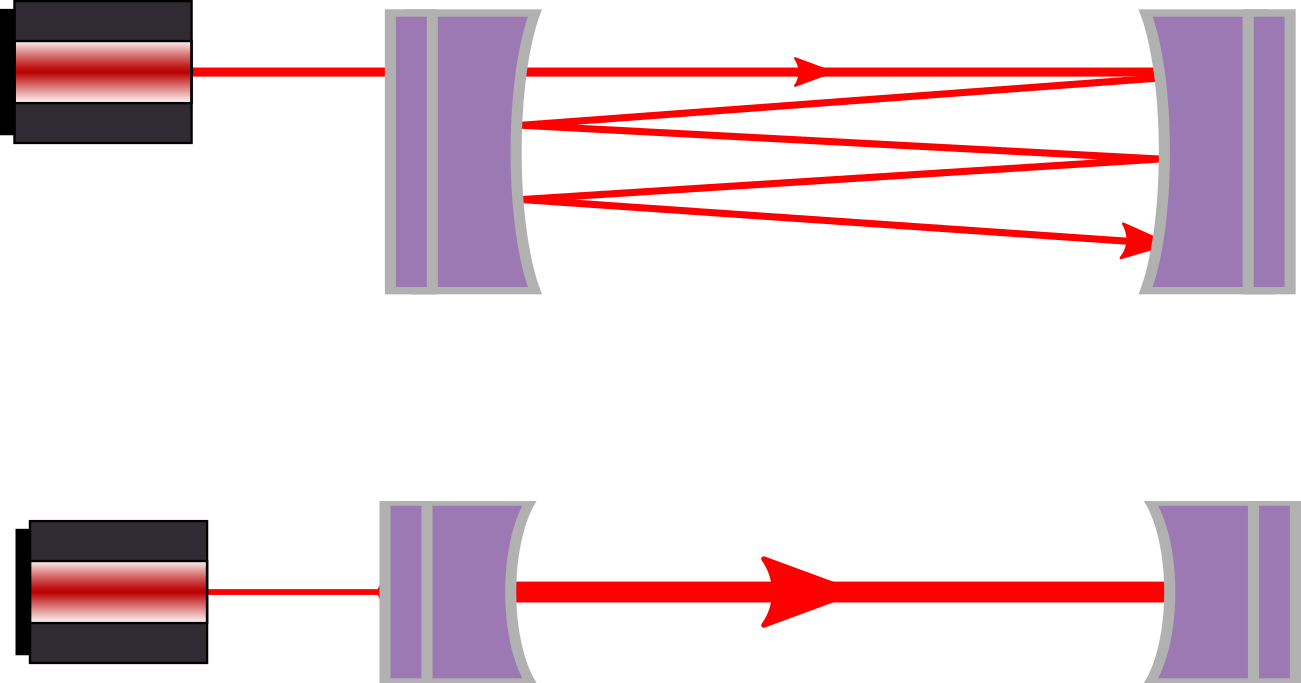
\includegraphics[width=.5 \textwidth]{../Figures/FPvDL.png}
		\caption{Delay Line vs Fabry Perot}
		\label{fig:FPvDL}
		\end{figure}
		
	
		A Fabry-Perot cavity is an optical system comprised of two or more partially transmitting mirrors with one laser input.  To create a resonator, the user must design a system so that once the laser has made one round trip within the optical system, the shape and size of the beam is the same as when it started.  This may seem simple conceptually but in practice, controlling and sensing any optical cavity comes with a few challenges.
		
		To start understanding the longitudinal degree of freedom, consider a two mirror system in Figure [FabryPerotFig] which is separated by a length $L$ with reflection and transmission coefficients: $r_1$, $t_1$, $r_2$, $t_2$.	
		Starting with a plane wave at the input mirror with amplitude $E_0$, the beam will enter the cavity and propagate back between the two mirrors.  The reflected, transmitted, and circulating fields \cite{Saulson}, which are a result of the geometric series, can be described as
		\begin{equation}\label{r_FP}
		E_{REFL} = r_{FP} E_0 = \bigg(-r_1 + \frac{t_1^2 r_2  e^{-i2kL}}{1-r_1 r_2 e^{-i2kL}} \bigg) E_0
		\end{equation}
		\begin{equation}\label{t_FP}
		E_{TRAN} = t_{FP} E_{0} = \bigg( \frac{t_1 t_2 e^{ikL}}{1-r_1 r_2 e^{-i2kL}}\bigg) E_0
		\end{equation}
		\begin{equation}\label{c_FP}
		E_{CIRC} = c_{FP} E_0 = \bigg(\frac{t_1}{1- r_1 r_2 e^{-2ikL}} \bigg) E_0
		\end{equation}
		The fields above are all highly dependent on the round trip phase and become resonant when the cavity length is $L = n \lambda / 2$ and the circulating coefficient in the cavity is maximized such that the gain is
		\begin{equation}
		\text{Gain} = c^2_{FP} \vert_{\text{resonating}} = \bigg( \frac{t_1}{1-r_1 r_2}\bigg)^2
		\end{equation}
		Depending on the relative reflection coefficients of the input and output mirrors, the fields on resonance will be slightly different Figure[UnderOverCritCoupled].
		
		\begin{figure}[ht]
			\centering
			\begin{subfigure}[b]{0.45\textwidth}
				\centering
				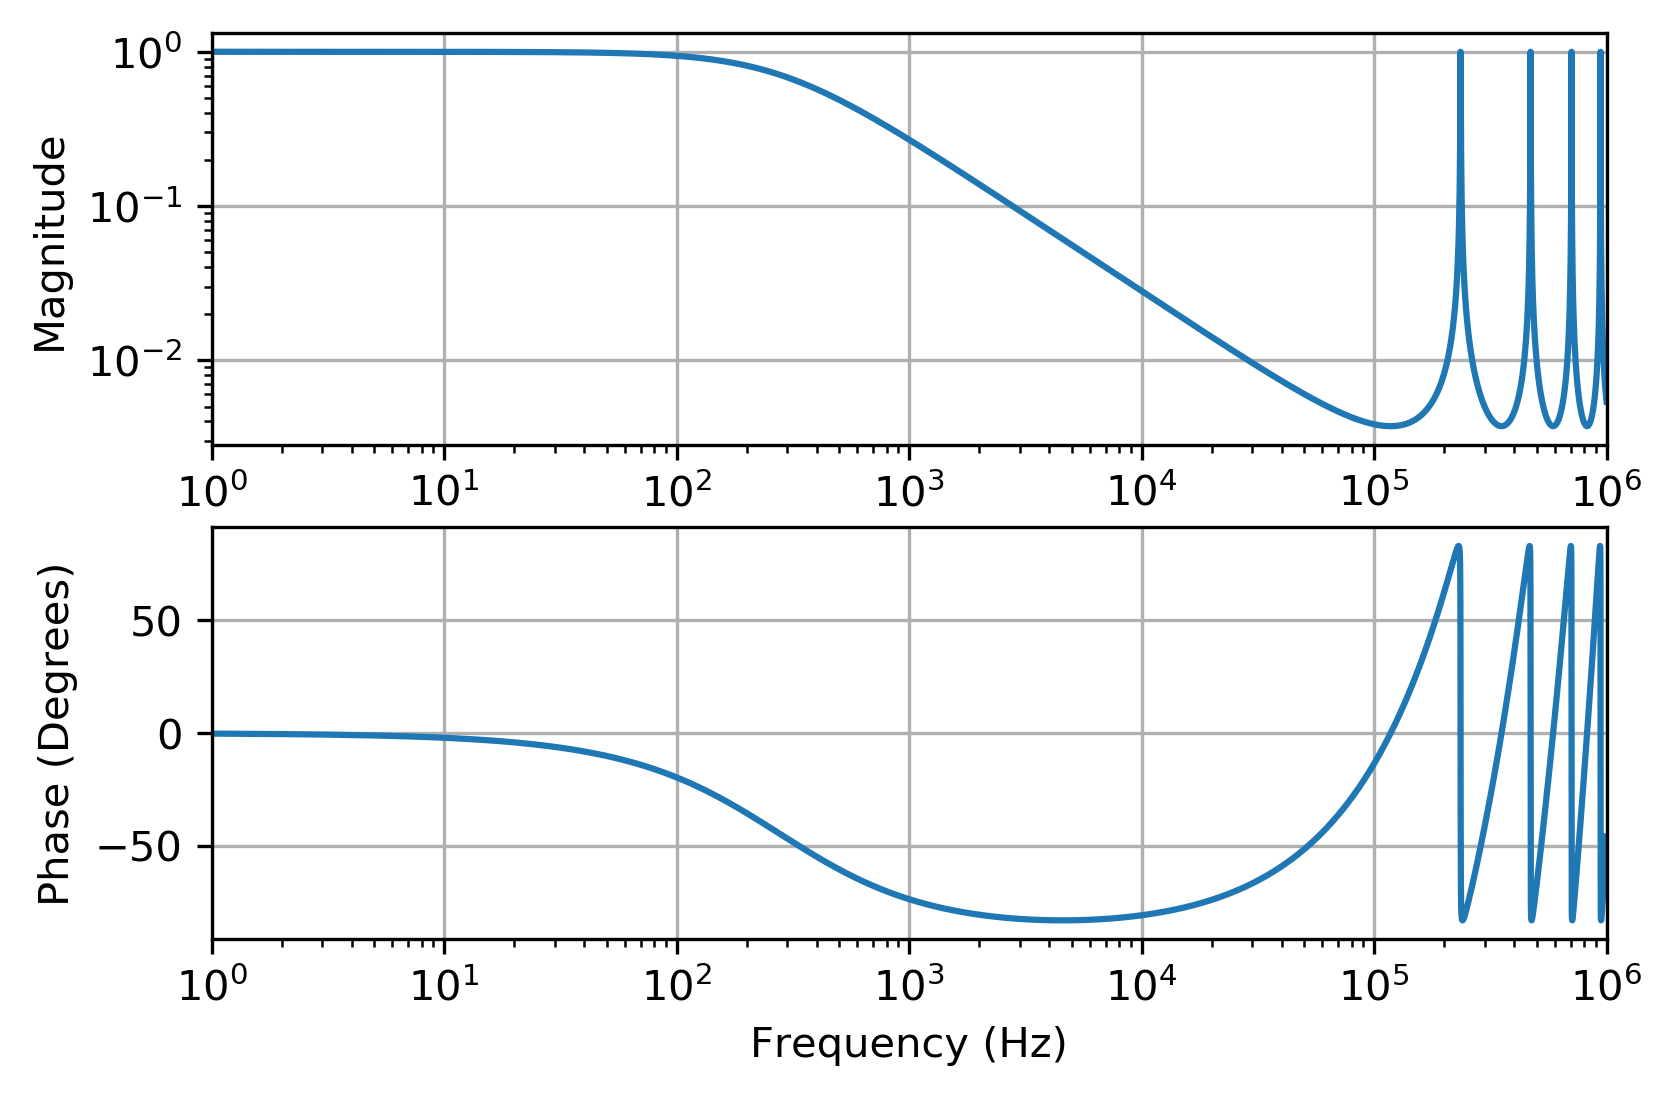
\includegraphics[width=\textwidth]{../Figures/FP_L_TF.png}
				\caption{Transfer function with respect to L}
				\label{fig:FP_L}
			\end{subfigure}
			\hfill
			\begin{subfigure}[b]{0.45\textwidth}
				\centering
				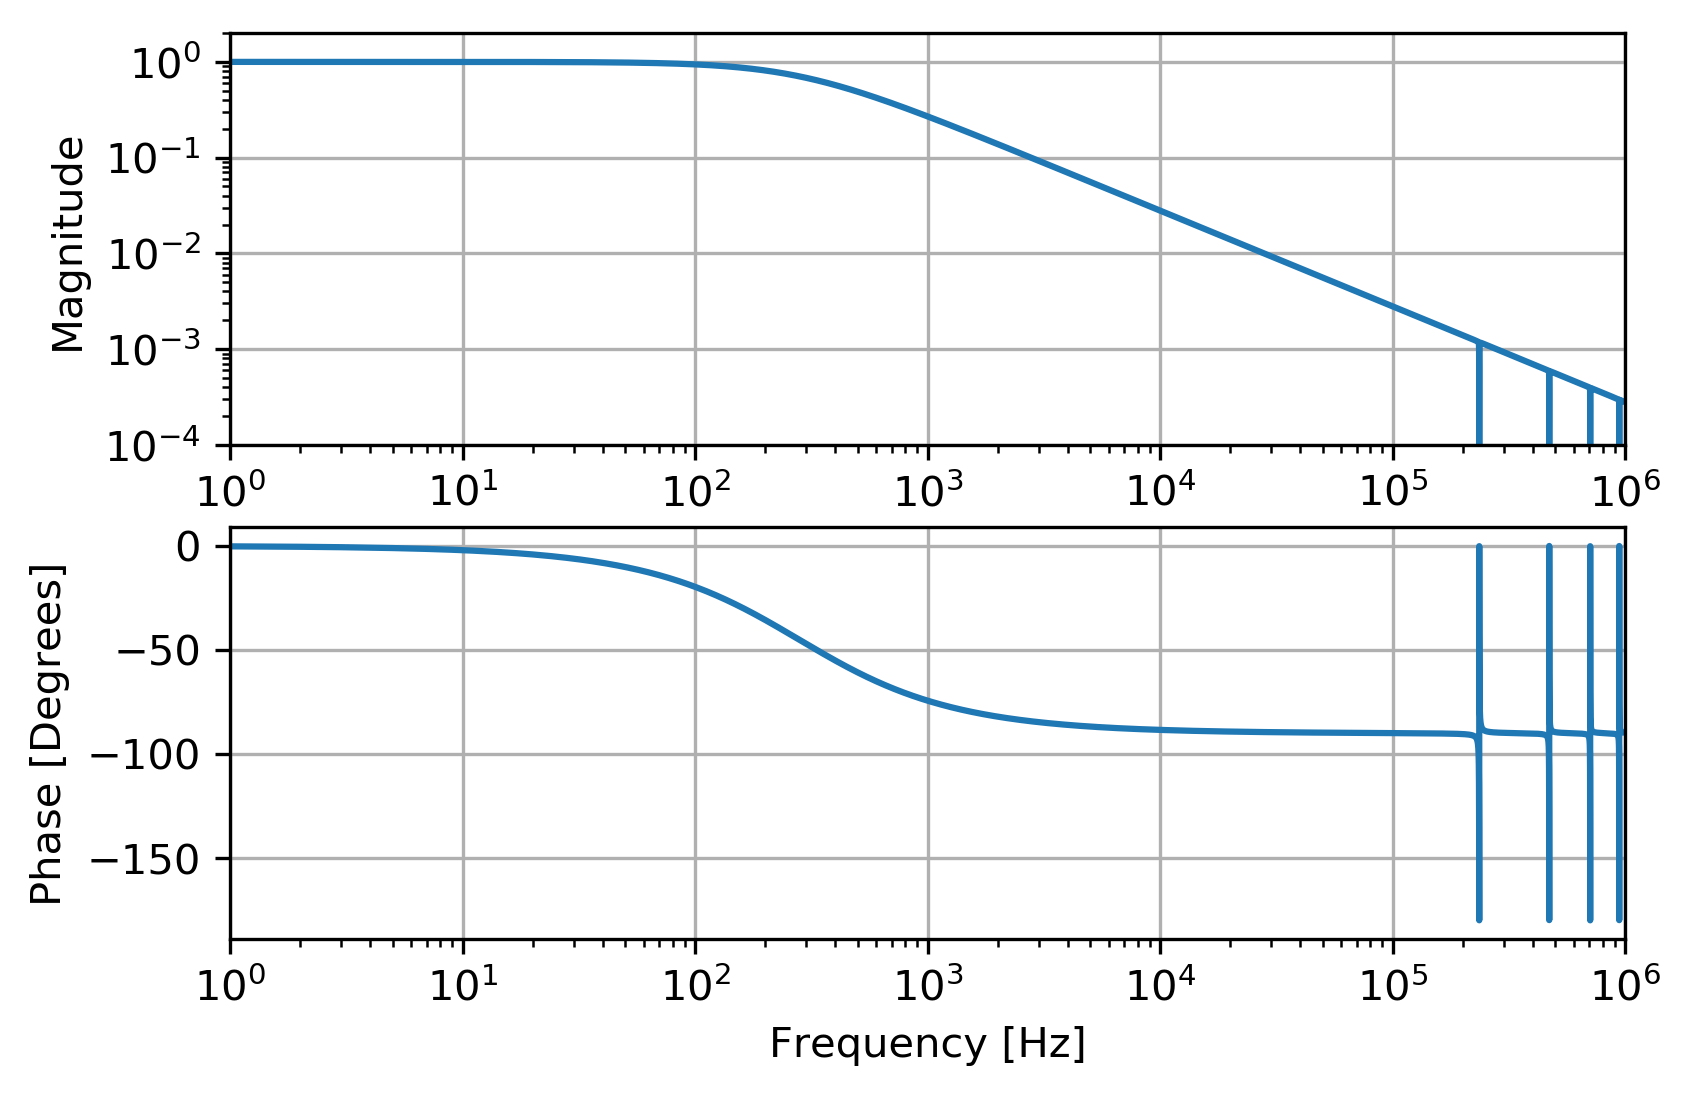
\includegraphics[width=\textwidth]{../Figures/FP_F_TF.png}
				\caption{Transfer function with respect to F}
				\label{fig:FP_F}
			\end{subfigure}
			\caption{Bode Plots of the Fabry Perot response}
			\label{fig:FP_Bode}
		\end{figure}
		
		Notice that the fields are dependent on the cavity length and laser frequency, $2kL$, so one might naively determine that modulating the two parameters independently cause the same effect.  However, when both are changing by large amounts, they are related by a frequency dependent transfer function 
		\begin{equation}
		C(s) \frac{\Delta w}{w} = -\frac{\Delta L}{L}
		\end{equation}
		where $C(s) = \frac{1-e^{-2sL/c}}{2sL/c}$ in the Laplace domain Figure[FreqRespFP]. Only when the cavity is on or near resonance, then the frequency and length variations are related by $\frac{\Delta w}{w} = -\frac{\Delta L}{L}$.
		
	
			\begin{figure}[ht]
		\centering
		\begin{subfigure}[b]{0.45\textwidth}
			\centering
			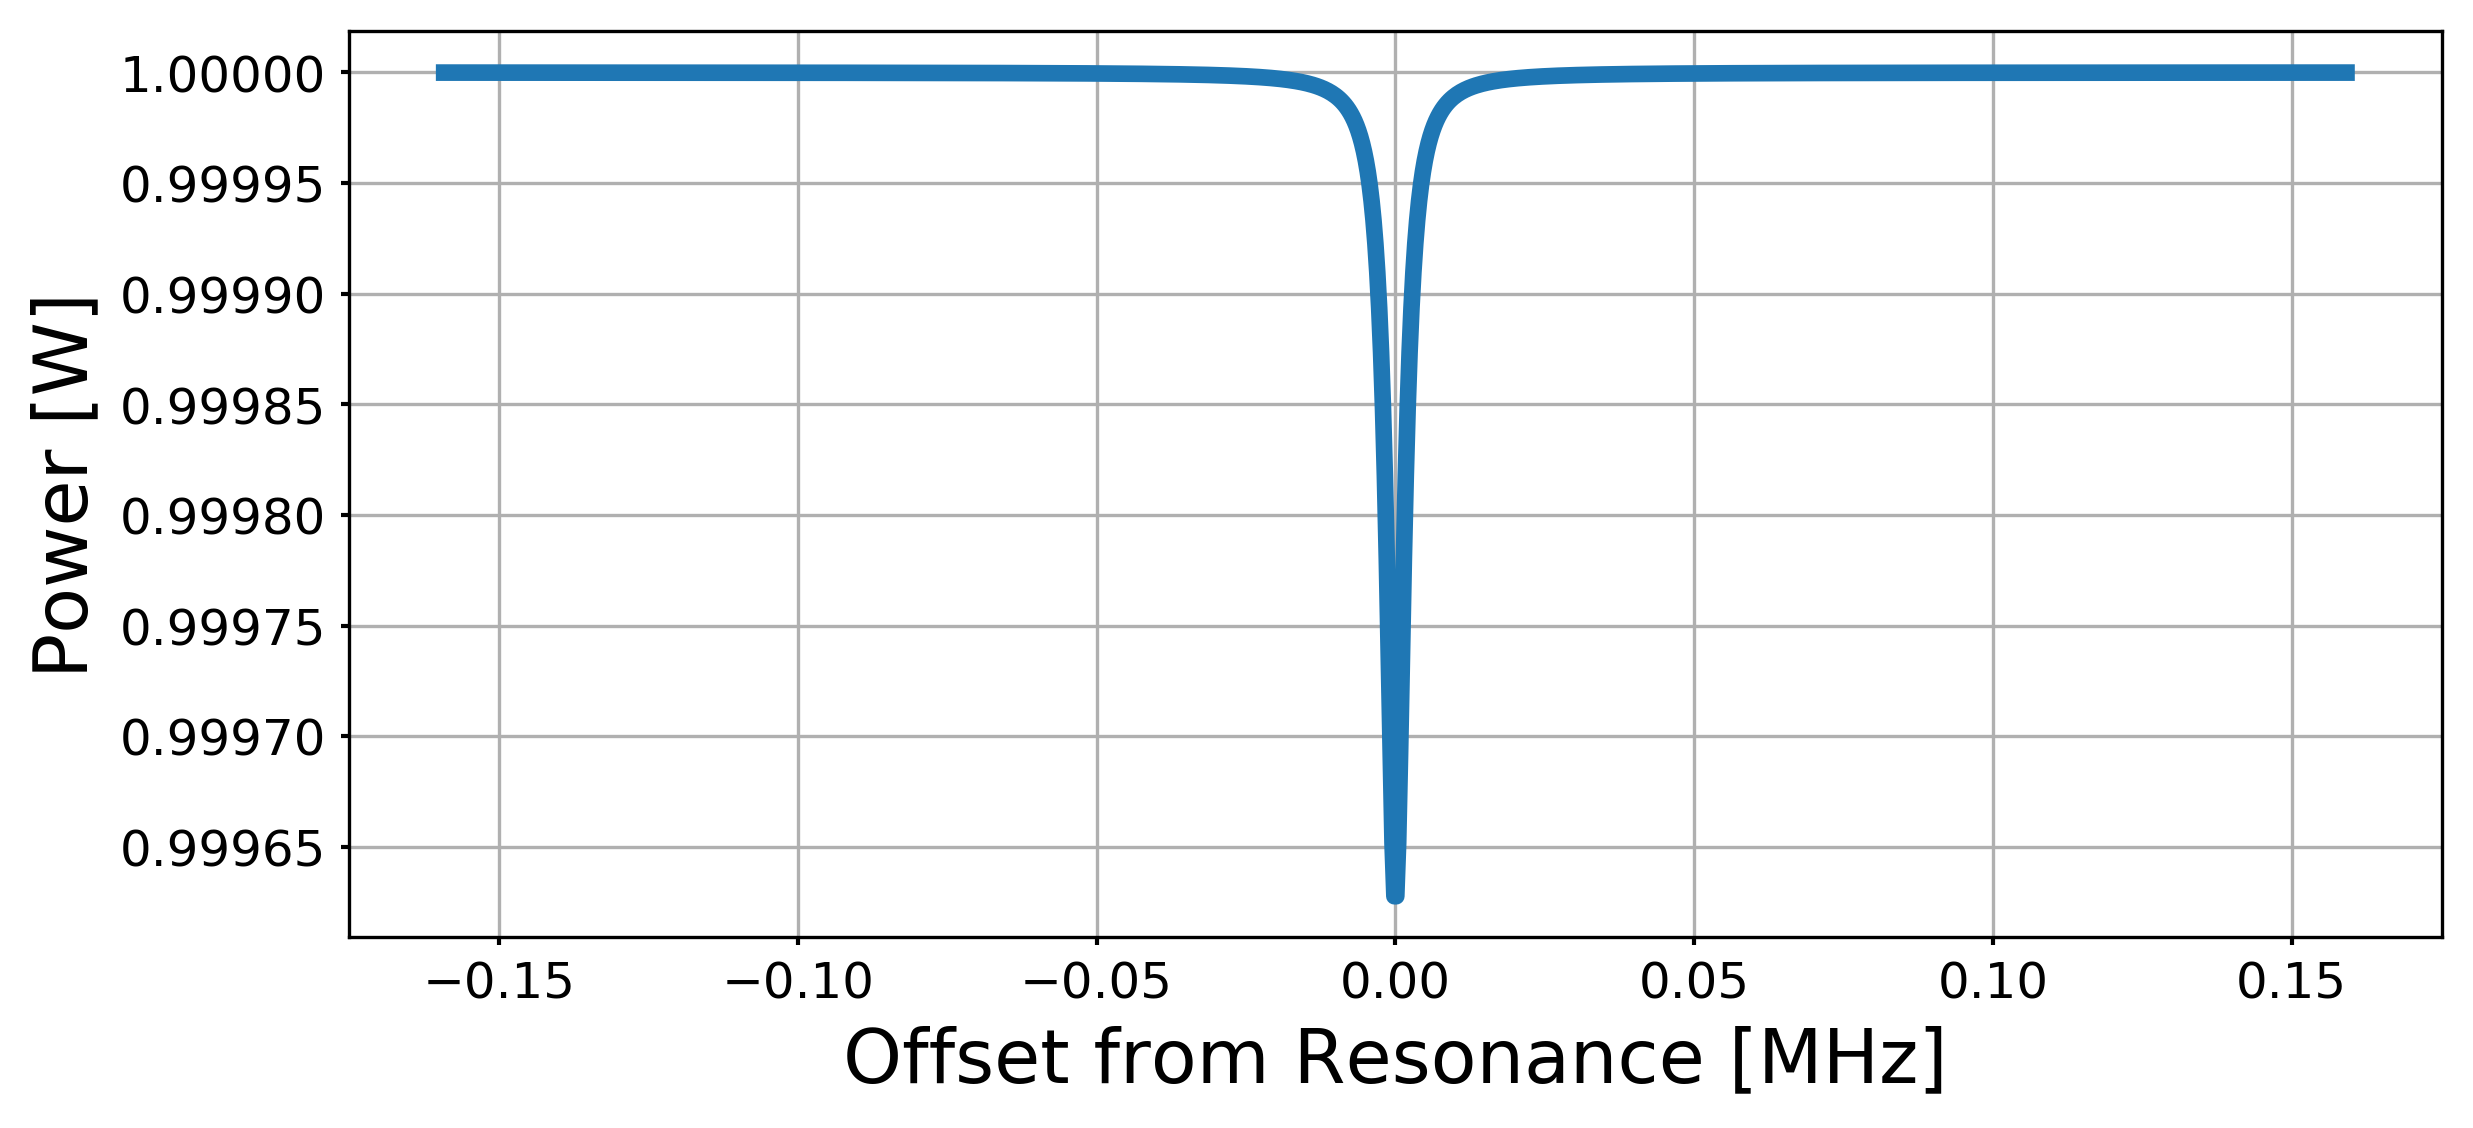
\includegraphics[width=\textwidth]{../Figures/Arm_Refl.png}
			\caption{Reflected Power}
			\label{fig:FP_refl}
		\end{subfigure}
		\hfill
		\begin{subfigure}[b]{0.45\textwidth}
			\centering
			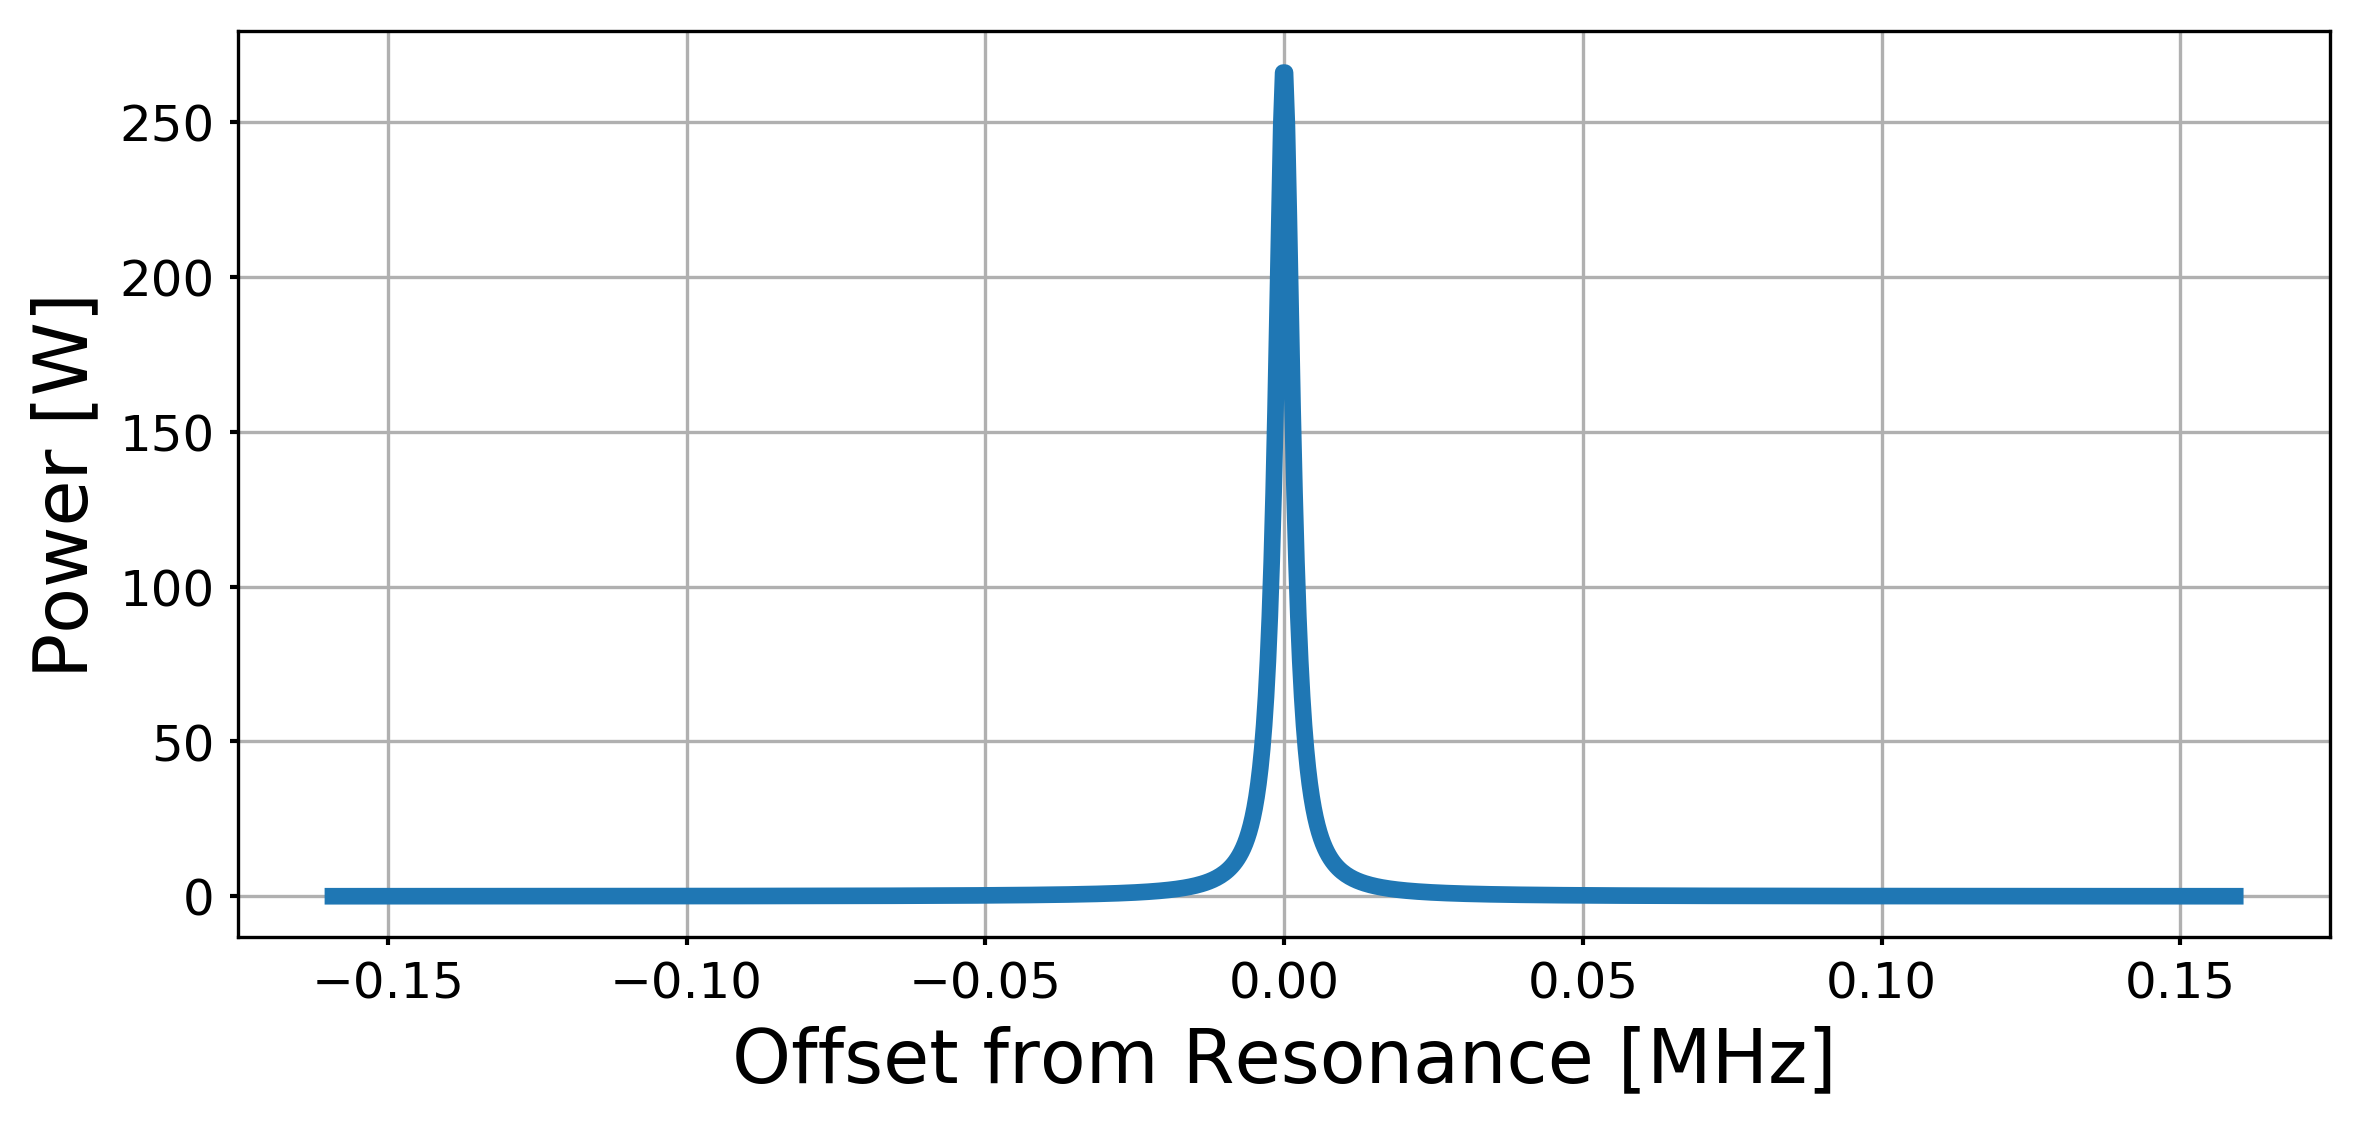
\includegraphics[width=\textwidth]{../Figures/Arm_Circ.png}
			\caption{Circulating Power}
			\label{fig:FP_circ}
		\end{subfigure}
		\hfill
		\begin{subfigure}[b]{0.45\textwidth}
			\centering
			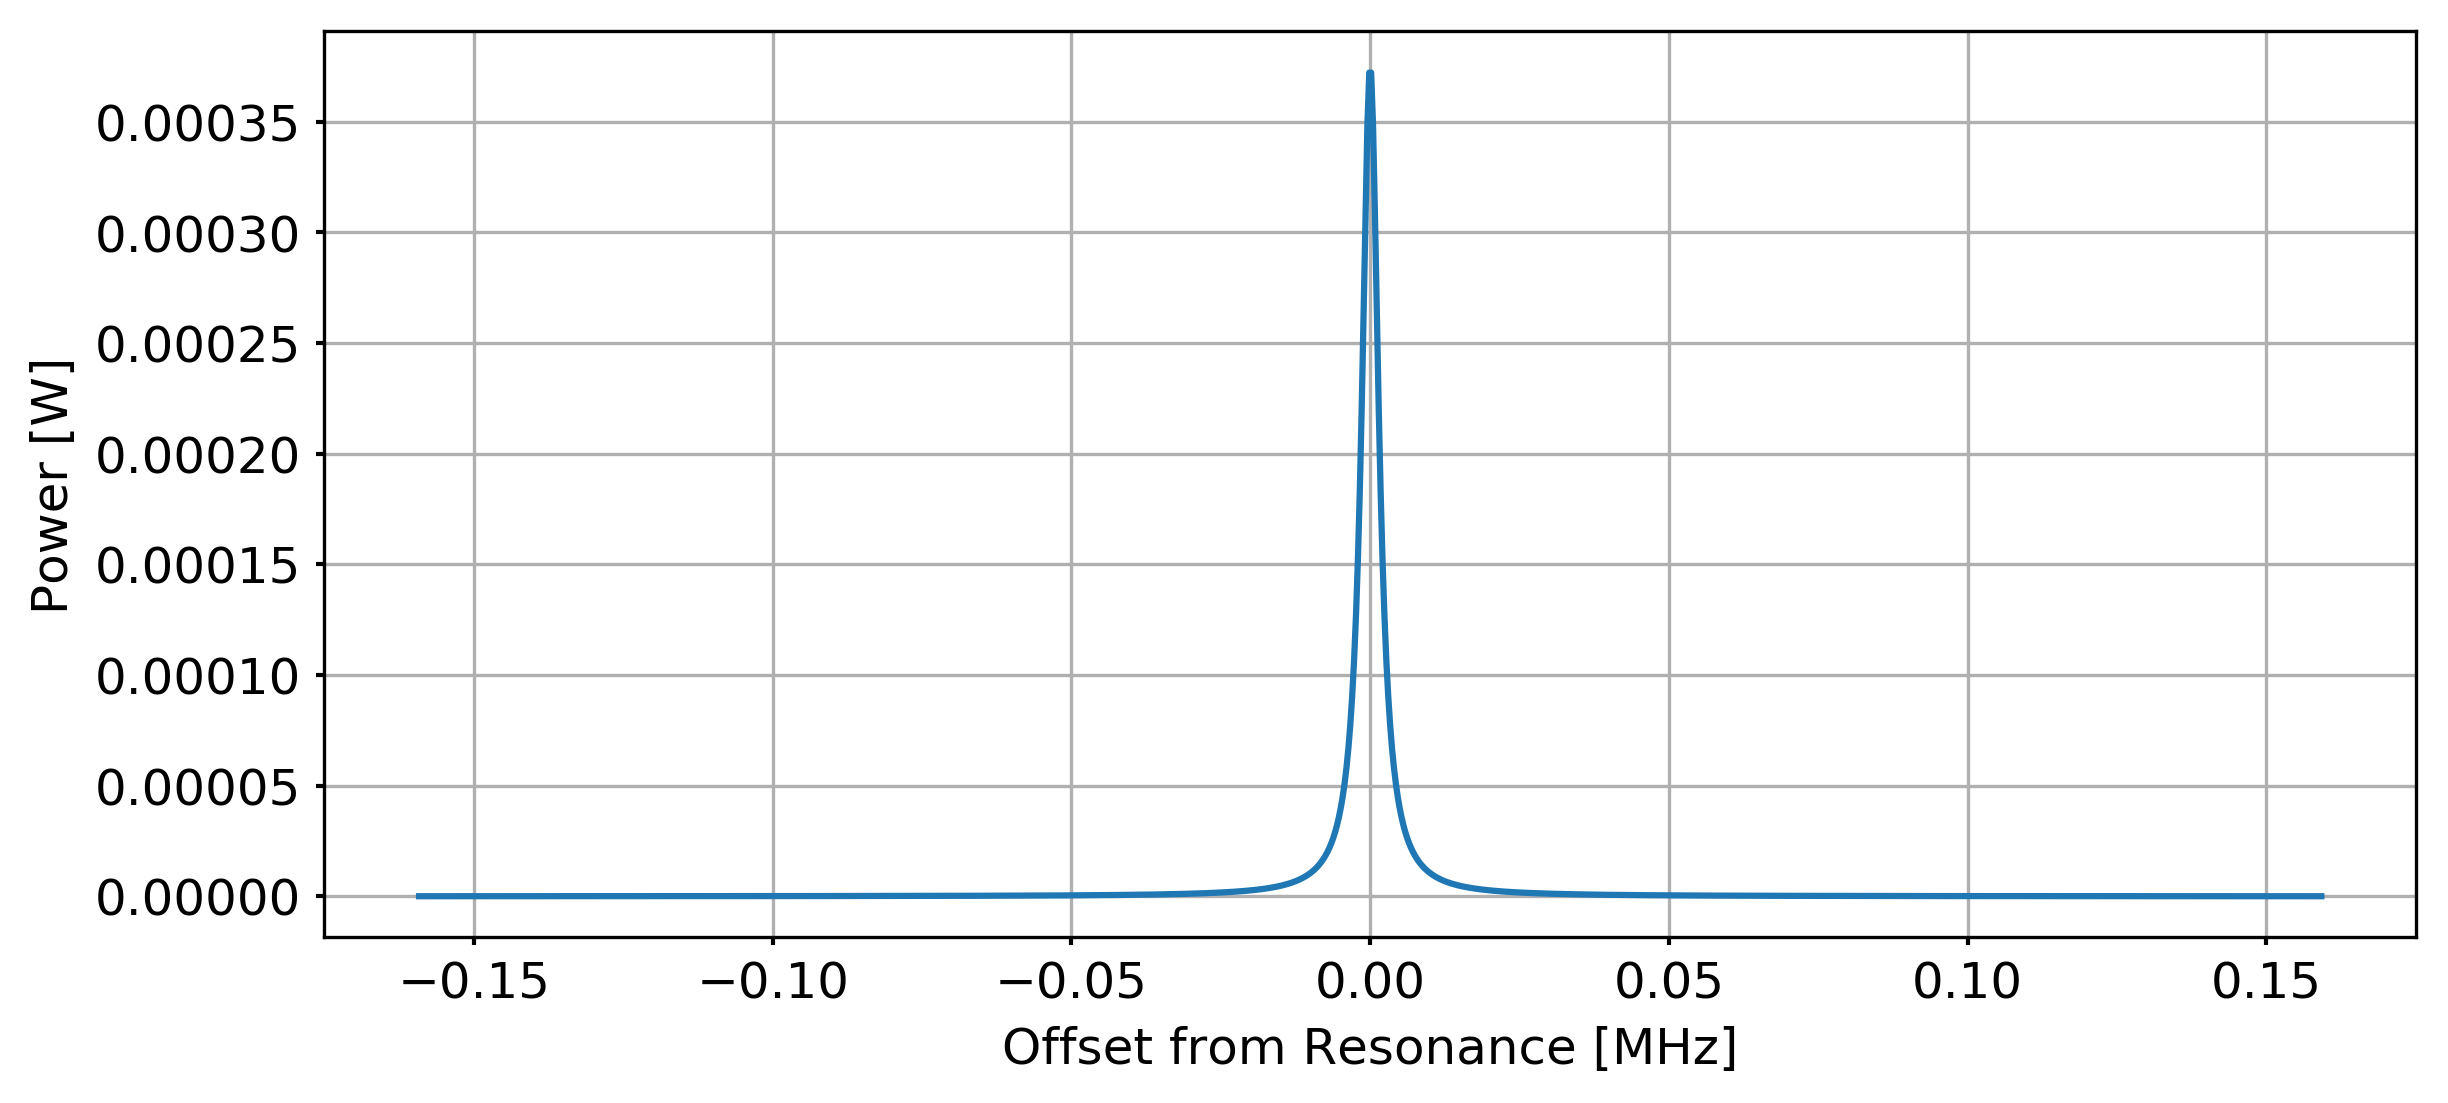
\includegraphics[width=\textwidth]{../Figures/Arm_Tran.png}
			\caption{Transmitted Power}
			\label{fig:FP_tran}
		\end{subfigure}
		\caption{The different powers for a single Fabry-Perot cavity that has properties in Table [] to represent one of the LIGO 4km arms which are highly over-coupled cavities so almost all of the light reflects toward the beamsplitter.  The input power is normalized to 1 Watt to show the relative gain of the circulating power.}
		\label{fig:FP_pwrs}
		\end{figure}
		
		While sweeping through either laser frequency or cavity length and measuring the reflected (or transmitted) fields, there are features of the power spectrum which relate directly to the cavity's physical properties:
		
		Finesse, or the line width of the resonant peak, function of $r_1$ and $r_2$:
		\begin{equation}\label{finesse}
		\mathbb{F} = \frac{\pi \sqrt{r_1 r_2}}{1- r_1 r_2}
		\end{equation}
		Storage Time :
		\begin{equation}
		\tau_{s} = \frac{L}{c \pi} \, \mathbb{F}
		\end{equation}
		Cavity Pole:
		\begin{equation}
		f_{pole} = \frac{1}{4\pi \tau_{s}}
		\end{equation}
		Free Spectral Range:
		\begin{equation}
		f_{FSR}  = \frac{c}{2L}
		\end{equation}

		Stability: In order to prove that an optical cavity is stable, it is useful to introduce the matrices that describe a periodic optical system which is explicitly derived in appendix \ref{FPappendix}.  A Fabry Perot cavity that is separated by distance $L$ with spherical mirrors that have radii of curvature $R_1$ and $R_2$ will need to satisfy 
		\begin{equation}\label{gfactor}
		0 \geq \bigg(1+\frac{L}{R_1}\bigg) \bigg(1+\frac{L}{R_2}\bigg) \geq 1
		\end{equation}
		in order to be geometrically stable (see Figure[BeamGeometryFP]).
		
		Power circulating as a function of our defined parameters slightly off resonance by a length of $\delta L$:
		\begin{equation}
		P_{cav} = \vert c_{FP} \vert^2 = \frac{\text{Gain}}{ 1 + \big(\frac{2\mathbb{F}}{\pi} \big)^2 \, \text{sin}^2(k \delta L) }
		\end{equation}
		
		LIGO uses the frequency response of optical cavities for a number of reasons: Firstly, the round trip phase of the gravitational wave is amplified by the finesse (equation \ref{finesse}) of the 4 kilometer arm cavities, therefore increasing the sensitivity.  Secondly, the input and output of the interferometer's Gaussian beam mode can be refined by only allowing the fundamental mode of the laser to resonate (input and output mode cleaners).  Thirdly, Advanced LIGO uses a dual-recycled Michelson interferometer which means the symmetric port has a mirror inserted to resonate the light reflected from the Fabry Perot arms (power recycling) and another mirror shapes the frequency response of the differential cavity pole at the anti-symmetric port (signal recycling).
		\subsubsection{Achieving Resonance in an Optical Cavity}
		Described above are the theoretical constructs of a FP cavity, but the question remains, how does one practically construct a resonant optical cavity?  The answer comes from using a heterodyne sensing scheme similar to the one described in Section \ref{michelson}.  Except the optical system is not a Michelson interferometer but rather a two mirror cavity.  Still, the heterodyne detection method can apply to a number of different geometries such as triangular or bow-tie cavities shown in Figure[DiffResCavs].
		
		Starting with an input laser and EOM (electro-optical modulator) that imparts upper and lower sidebands at a modulation frequency $\Omega$, the user injects three beams into the optical system described in Equation \ref{modE}.  When placing a photodetector on the reflection port, one should see the cavity's effect on each of the three electric fields.
		
		\begin{equation}
		E_{FP,out} = E_{C} + E_{SB+} + E_{SB-} = 
		\begin{pmatrix}
		r_{C} 	&   
		\\ 	r_{SB+} &
		\\ 	r_{SB-} &
		\end{pmatrix}
		\begin{pmatrix}
		E_{C,in} &    E_{SB+,in}    &  E_{SB-,in}     
		\end{pmatrix}
		\end{equation}
		
		where the reflection coefficients follow equation \ref{r_FP}.  Because sidebands are frequency shifted, they will effectively $see$ a different cavity than the carrier and the total phase accumulated between the fields will be different. To make a good reference for the resonant carrier beam, the modulation frequency, $k_{\Omega}$, is chosen such that sidebands are be anti-resonant in the cavity.  
		\begin{equation}
		r_{C} = -r_1 + \frac{t_1^2 r_2  e^{-i2kL}}{1-r_1 r_2 e^{-i2kL}}
		\end{equation}
		and 
		\begin{equation}
		r_{SB\pm} = -r_1 + \frac{t_1^2 r_2  e^{-i2(k+k_{\Omega})L}}{1-r_1 r_2 e^{-i2(k+k_{\Omega})L}}
		\end{equation}
		The formalism to read out the error signal is the shown in Equation \ref{RFdet}. Using a photodetector in reflection (see Figure \ref{fig:FPControl}), the error signal will be linearly proportional to the laser frequency and cavity length \cite{BlackPDH}.
		\begin{equation}
		\text{Error Signal} \propto \frac{L \mathbb{F}}{\lambda} \bigg[\frac{\delta w}{w} + \frac{\delta L}{L}\bigg]
		\end{equation}
		
		\begin{figure}[h]
		\centering
		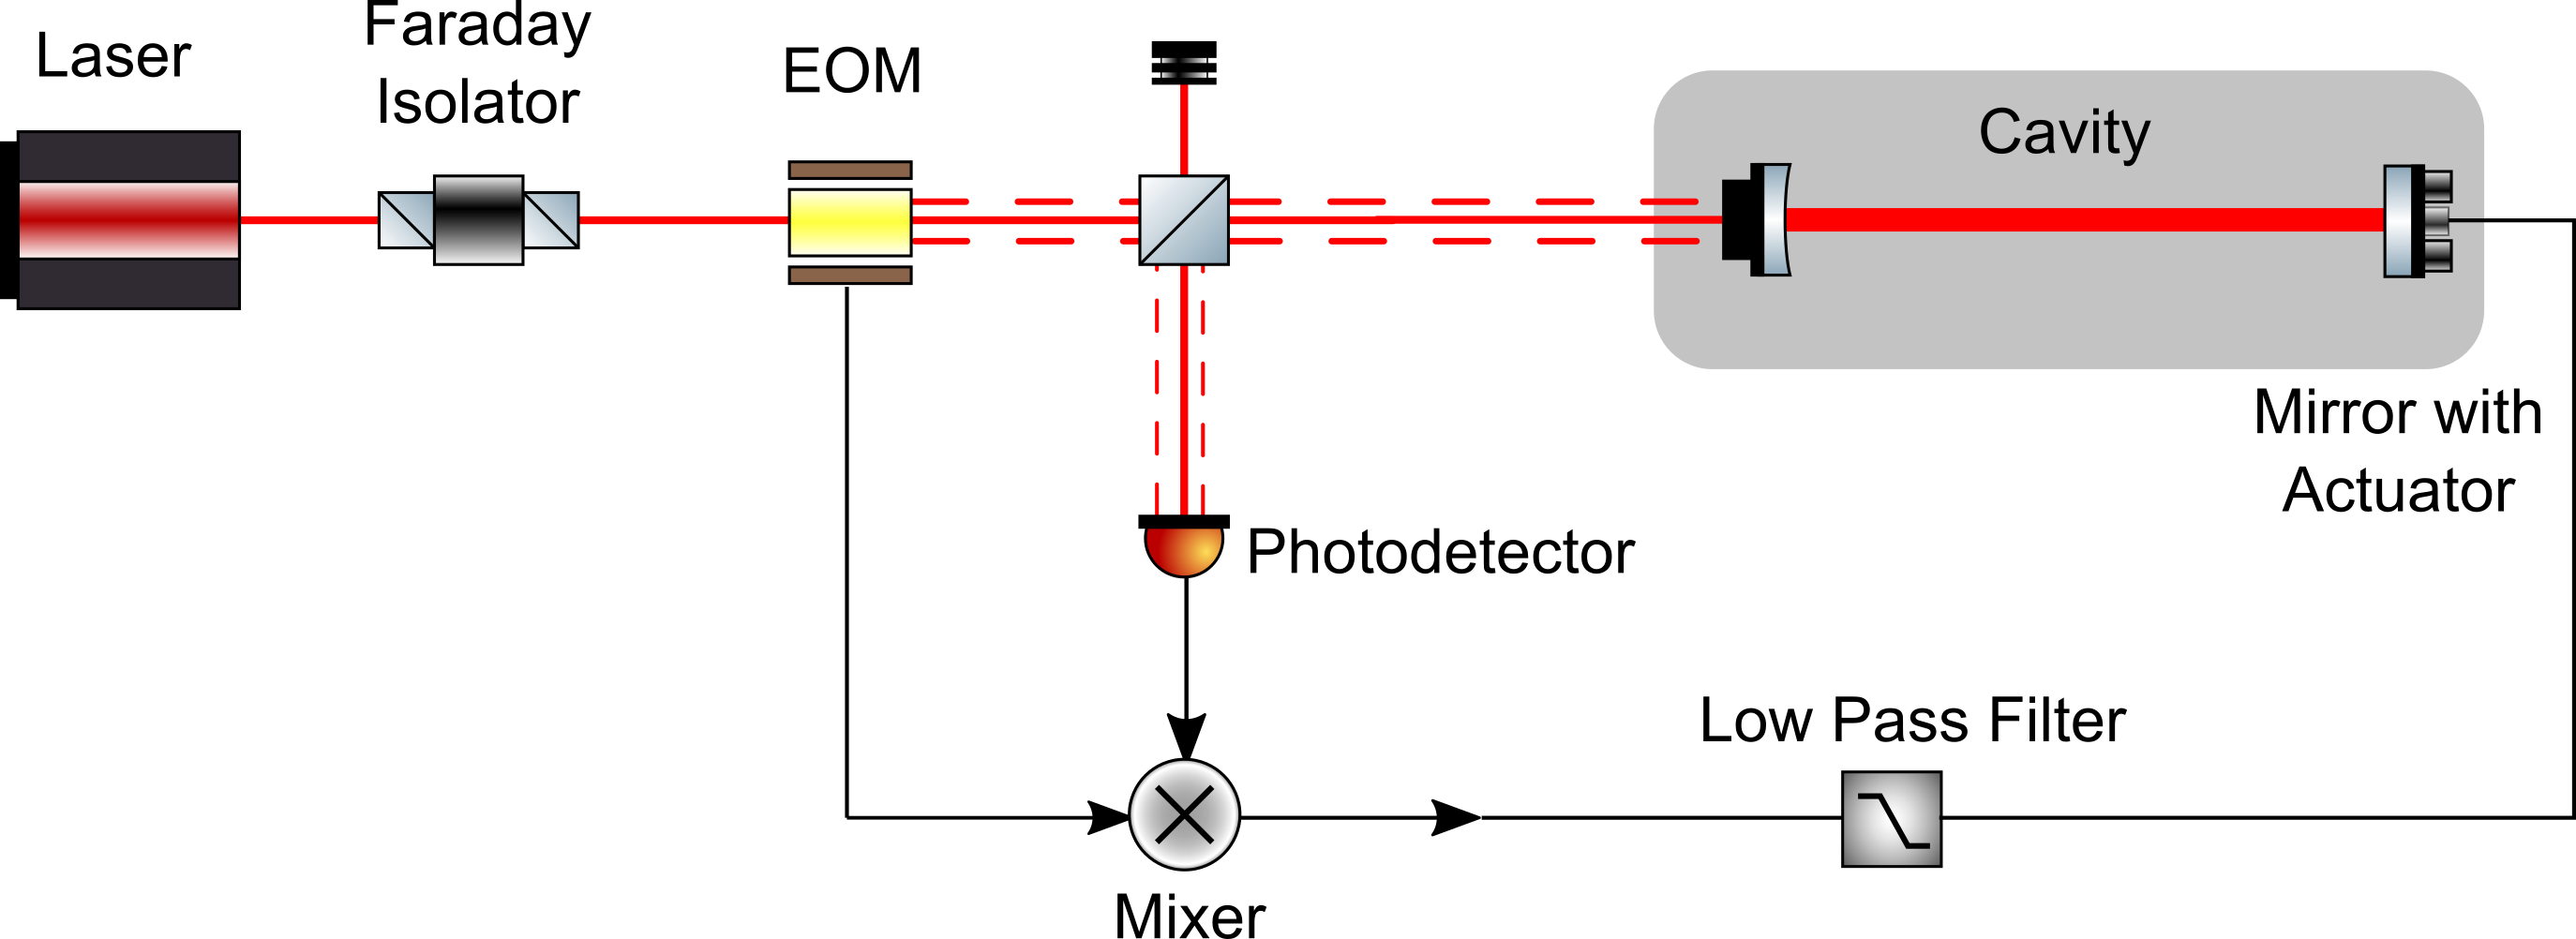
\includegraphics[width=.75 \textwidth]{../Figures/FP_Control.png}
		\caption{Control scheme for an optical cavity.}
		\label{fig:FPControl}
		\end{figure}
	
		\begin{figure}[h]
		\centering
		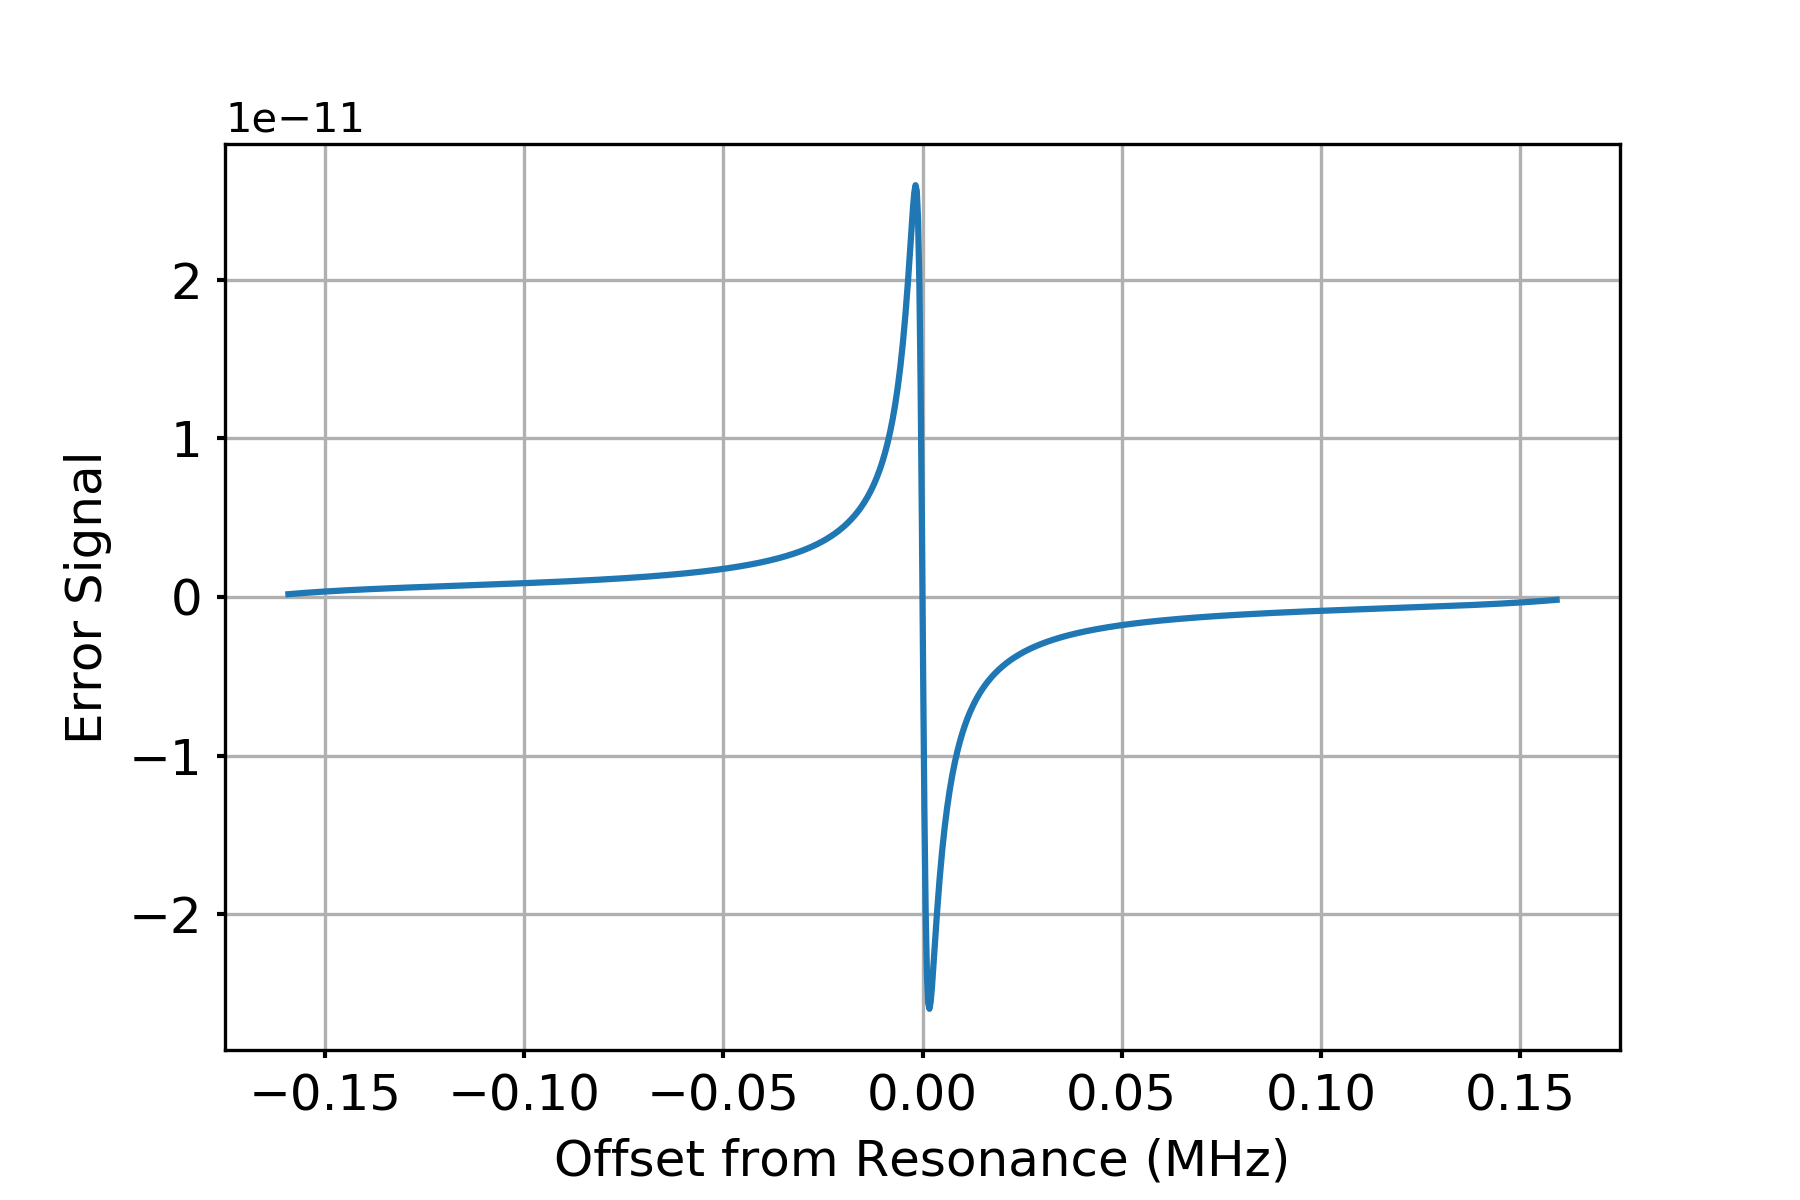
\includegraphics[width=.75 \textwidth]{../Figures/PDH_Err.png}
		\caption{Error signal in reflection}
		\label{fig:FP_err}
		\end{figure}
	
		
		\subsection{Fabry-Perot Michelson}\label{FPmich}
		Using an optical cavity to increase the number of bounces along the 4 kilometer arms will amplify the gravitational wave signal but it will also shape the frequency dependence of the sensitivity as well.  This has already been alluded to in section \ref{measuringGWs} where the overall increase in arm length will tune the response function of equation \ref{gwsinc}.  The same formalism can apply to integrate the use of Fabry-Perot arms into a Michelson interferometer and looking at the signal at the antisymmetric port as a function of gravitational wave frequency. Previously in section \ref{michelson}, it was shown that the RF detection technique required beating the sidebands with a carrier field containing the gravitational wave information.  However, this is not exclusively true because the signal sidebands beating with a reference carrier field could also be a valid way of measuring a signal of interest. In fact, Advanced LIGO employs a homodyne detection called DC readout \cite{FritschelReadout}\cite{FritschelAdvancedLIGO}. The idea is that the carrier field will resonant in the arms but will be slightly modulated due to a gravitational wave.  In effect, the carrier will have audio frequency sidebands imparted on the field shown in Figure[gwsb].  
		
		Figure \ref{fig:FPMichelson} shows an input electric field of $E_0$ incident on a 50/50 beamsplitter which then enters two orthogonal arm cavities of length $L_x$ and $L_y$.  Notice that the distance from the beamsplitter to the input couplers for both arms denoted by $l_x$ and $l_y$ are independent variables, this is to account for the DARM offset which is analogous to the Schnupp asymmetry described in section \ref{michelson}.  After partially transmitting and reflecting at the beamsplitter, the fields will resonate in each of the arm cavities and obey the reflectivity relations described by equation \ref{r_FP}.  Upon recombining at the beamsplitter, the antisymmetric port electric field will be related to the arm fields by,
		\begin{equation}
		E_{\text{AS}} = \frac{1}{\sqrt{2}} [E_{x}^{\text{ARM}} + E_{y}^{\text{ARM}} ] 
		\end{equation}
		where $E_{i}^{\text{ARM}} = E(\omega) \pm [E(+ \omega_{\text{\tiny GW}}) + E(- \omega_{\text{\tiny GW}})] \sin{k\delta l } $ is the reflectionfig:FPMichelson coefficient for the x and y arms which contain the carrier(first term) and GW signal sidebands(last two terms).  Intuitively, one can deduce that the antisymmetric port will only be sensitive to the differential motion between the arm cavities, which means the gravitational wave sidebands in the x-arm will be out of phase with the y-arm.  Also it is important to note that inserting a DC microscopic length shift, $\delta l = l_x - l_y$ allows for some carrier leakage field to propagate towards the antisymmetric port which creates a static reference to form a beat note with the signal sidebands.  The same effect can be achieved by introducing a static offset between the x and y arms; colloquially, this is referred to as DARM offset.
				
		\begin{figure}[h]
			\centering
			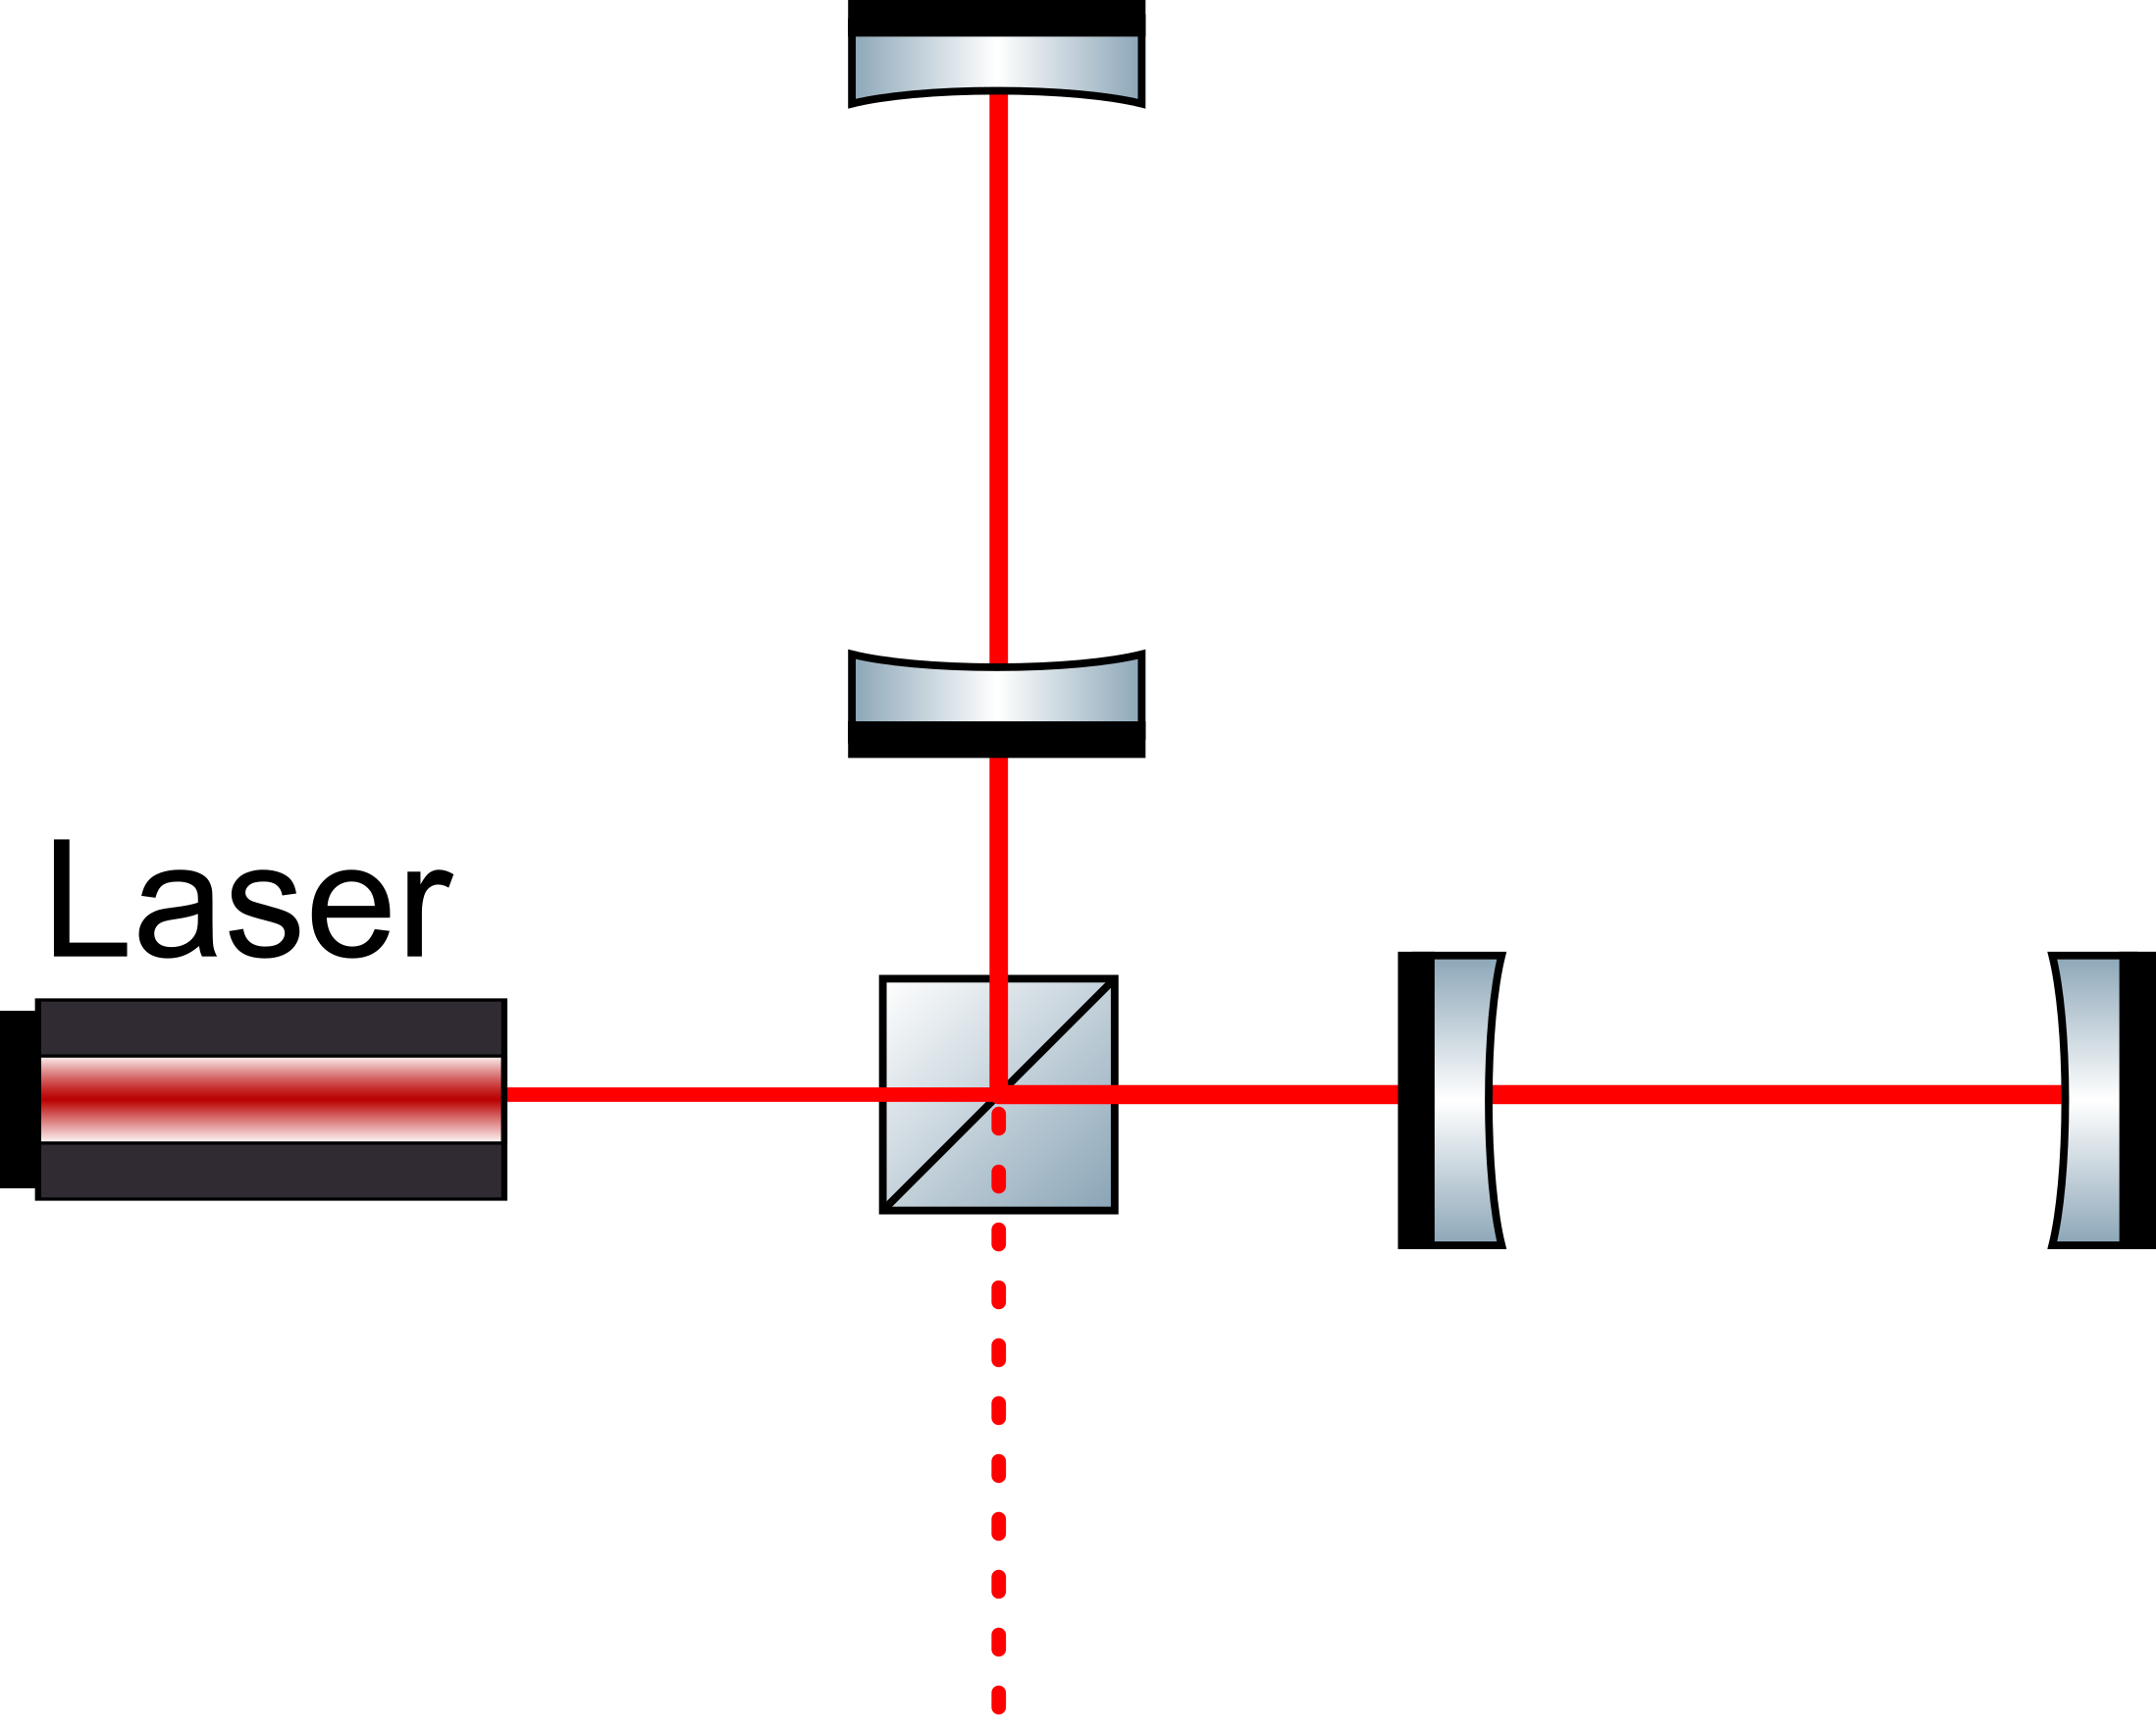
\includegraphics[width=.3 \textwidth]{../Figures/FP_Mich.png}
			\caption{Michelson with Fabry Perot arms}
			\label{fig:FPMichelson}
		\end{figure}
	
		For the carrier field, the amplitude of reflection is simple because the LIGO arms are a strongly overcoupled cavity operating on resonance therefore 
		\begin{equation}
			E(\omega) = \frac{E_0}{\sqrt{2}}  \bigg(-r_1 + \frac{t_1^2 r_2}{1-r_1 r_2} \bigg) \approx -\frac{E_0}{\sqrt{2}}
		\end{equation}
		
		The sidebands are a different story because the modulation caused by the gravitational wave slightly move the field off resonance.  Imagine the carrier circulating in the arms and then suddenly, a disturbance due to a gravitational wave displaces the end mirror at a frequency $\omega_\text{GW}$ by an amount $\Delta L$.   By using the same formalism as the expansion of a modulated field in equation \ref{modE}, the sideband fields can be described by,
		\begin{equation}
		\begin{aligned}\label{Egw}
			E(\pm \omega_{\text{\tiny GW}}) &= \bigg[ \frac{t_1}{1-r_1 r_2 e^{-2ikL}}\bigg] \frac{E_0}{\sqrt{2}} \bigg[\frac{t_1}{1-r_1 r_2 e^{-2i (kL \pm \omega_{\text{\tiny GW}}  \frac{L}{c})}} \bigg] ik\Delta L\\
			& =  \bigg[ \frac{t_1^2}{1-r_1 r_2}\bigg]  \frac{E_0}{\sqrt{2}} \bigg[\frac{ 1}{1-r_1 r_2 e^{-2i  \omega_{\text{\tiny GW}}  \frac{L}{c}}} \bigg] ik\Delta L
		\end{aligned}
		\end{equation}
		The first bracket is the circulating field of the carrier signal amplified by the Fabry Perot cavity and the second bracket is the circulating field slightly off resonance due to the gravitational wave frequency offset.  Setting the fields to resonate already simplifies the equation but it is also reasonable to approximate the gravitational wave as a weak signal and expand the exponential $e^{- 2i \omega_{\text{\tiny GW}}  \frac{L}{c}} \approx 1 - 2i \omega_{\text{\tiny GW}}  \frac{L}{c}$.  This transforms the signal sideband field into a simple form,
		\begin{equation}
		E(\pm \omega_{\text{\tiny GW}}) \approx \bigg[\frac{t_1}{1-r_1r_2}\bigg]^2 \, \frac{E_0}{\sqrt{2}} \, \bigg[\frac{1}{1 \pm i \frac{\omega_{\text{\tiny GW}}}{\omega_p}}\bigg] ik\Delta L
		\end{equation}
		where $\omega_p = \frac{1-r_1r_2}{r_1r_2}\frac{c}{2L}$ is the differential pole frequency; notice that it matches the single arm cavity pole.
		
		The photodiode signal at the antisymmetric port is proportional to the beat note between the carrier and signal sideband that is demodulated in the audio band with a phase $\phi_{D}$,
		\begin{equation}
		\begin{aligned}
			S &\propto 2 [E(\omega) E^*(+\omega_{\text{\tiny GW}}) +  E(-\omega_{\text{\tiny GW}}) E^*(\omega) ] \sin{(k\delta l)} \sin{(\phi_{D})} \\
			  &\propto E_0^2 \; \frac{8\pi L}{\lambda}  \bigg[\frac{t_1}{1-r_1r_2}\bigg]^2 \bigg[\frac{1}{1 - i \frac{\omega_{\text{\tiny GW}}}{\omega_p}}\bigg] \sin{(k\delta l)} \sin{(\phi_{D})} h_{\text{\tiny GW}}
		\end{aligned}
		\end{equation}
		where the length disturbance $\Delta L$ was transformed to originate from a gravitational wave signal $k \Delta L = \frac{2\pi L}{\lambda} h_{\text{\tiny GW}}$.
		The response in this particular interferometer setup to the presence of differential length motion is linearly proportional to the gravitational wave amplitude as well as the input power $P_0 = E_0^2$, but there is also a frequency dependent component which is the same as a single Fabry-Perot arm that acts like a low pass filter above the corner frequency.

		\subsection{Power-Recycled Fabry-Perot Interferometers}
		
		\begin{figure}[ht]
			\centering
			\begin{subfigure}[b]{0.3\textwidth}
				\centering
				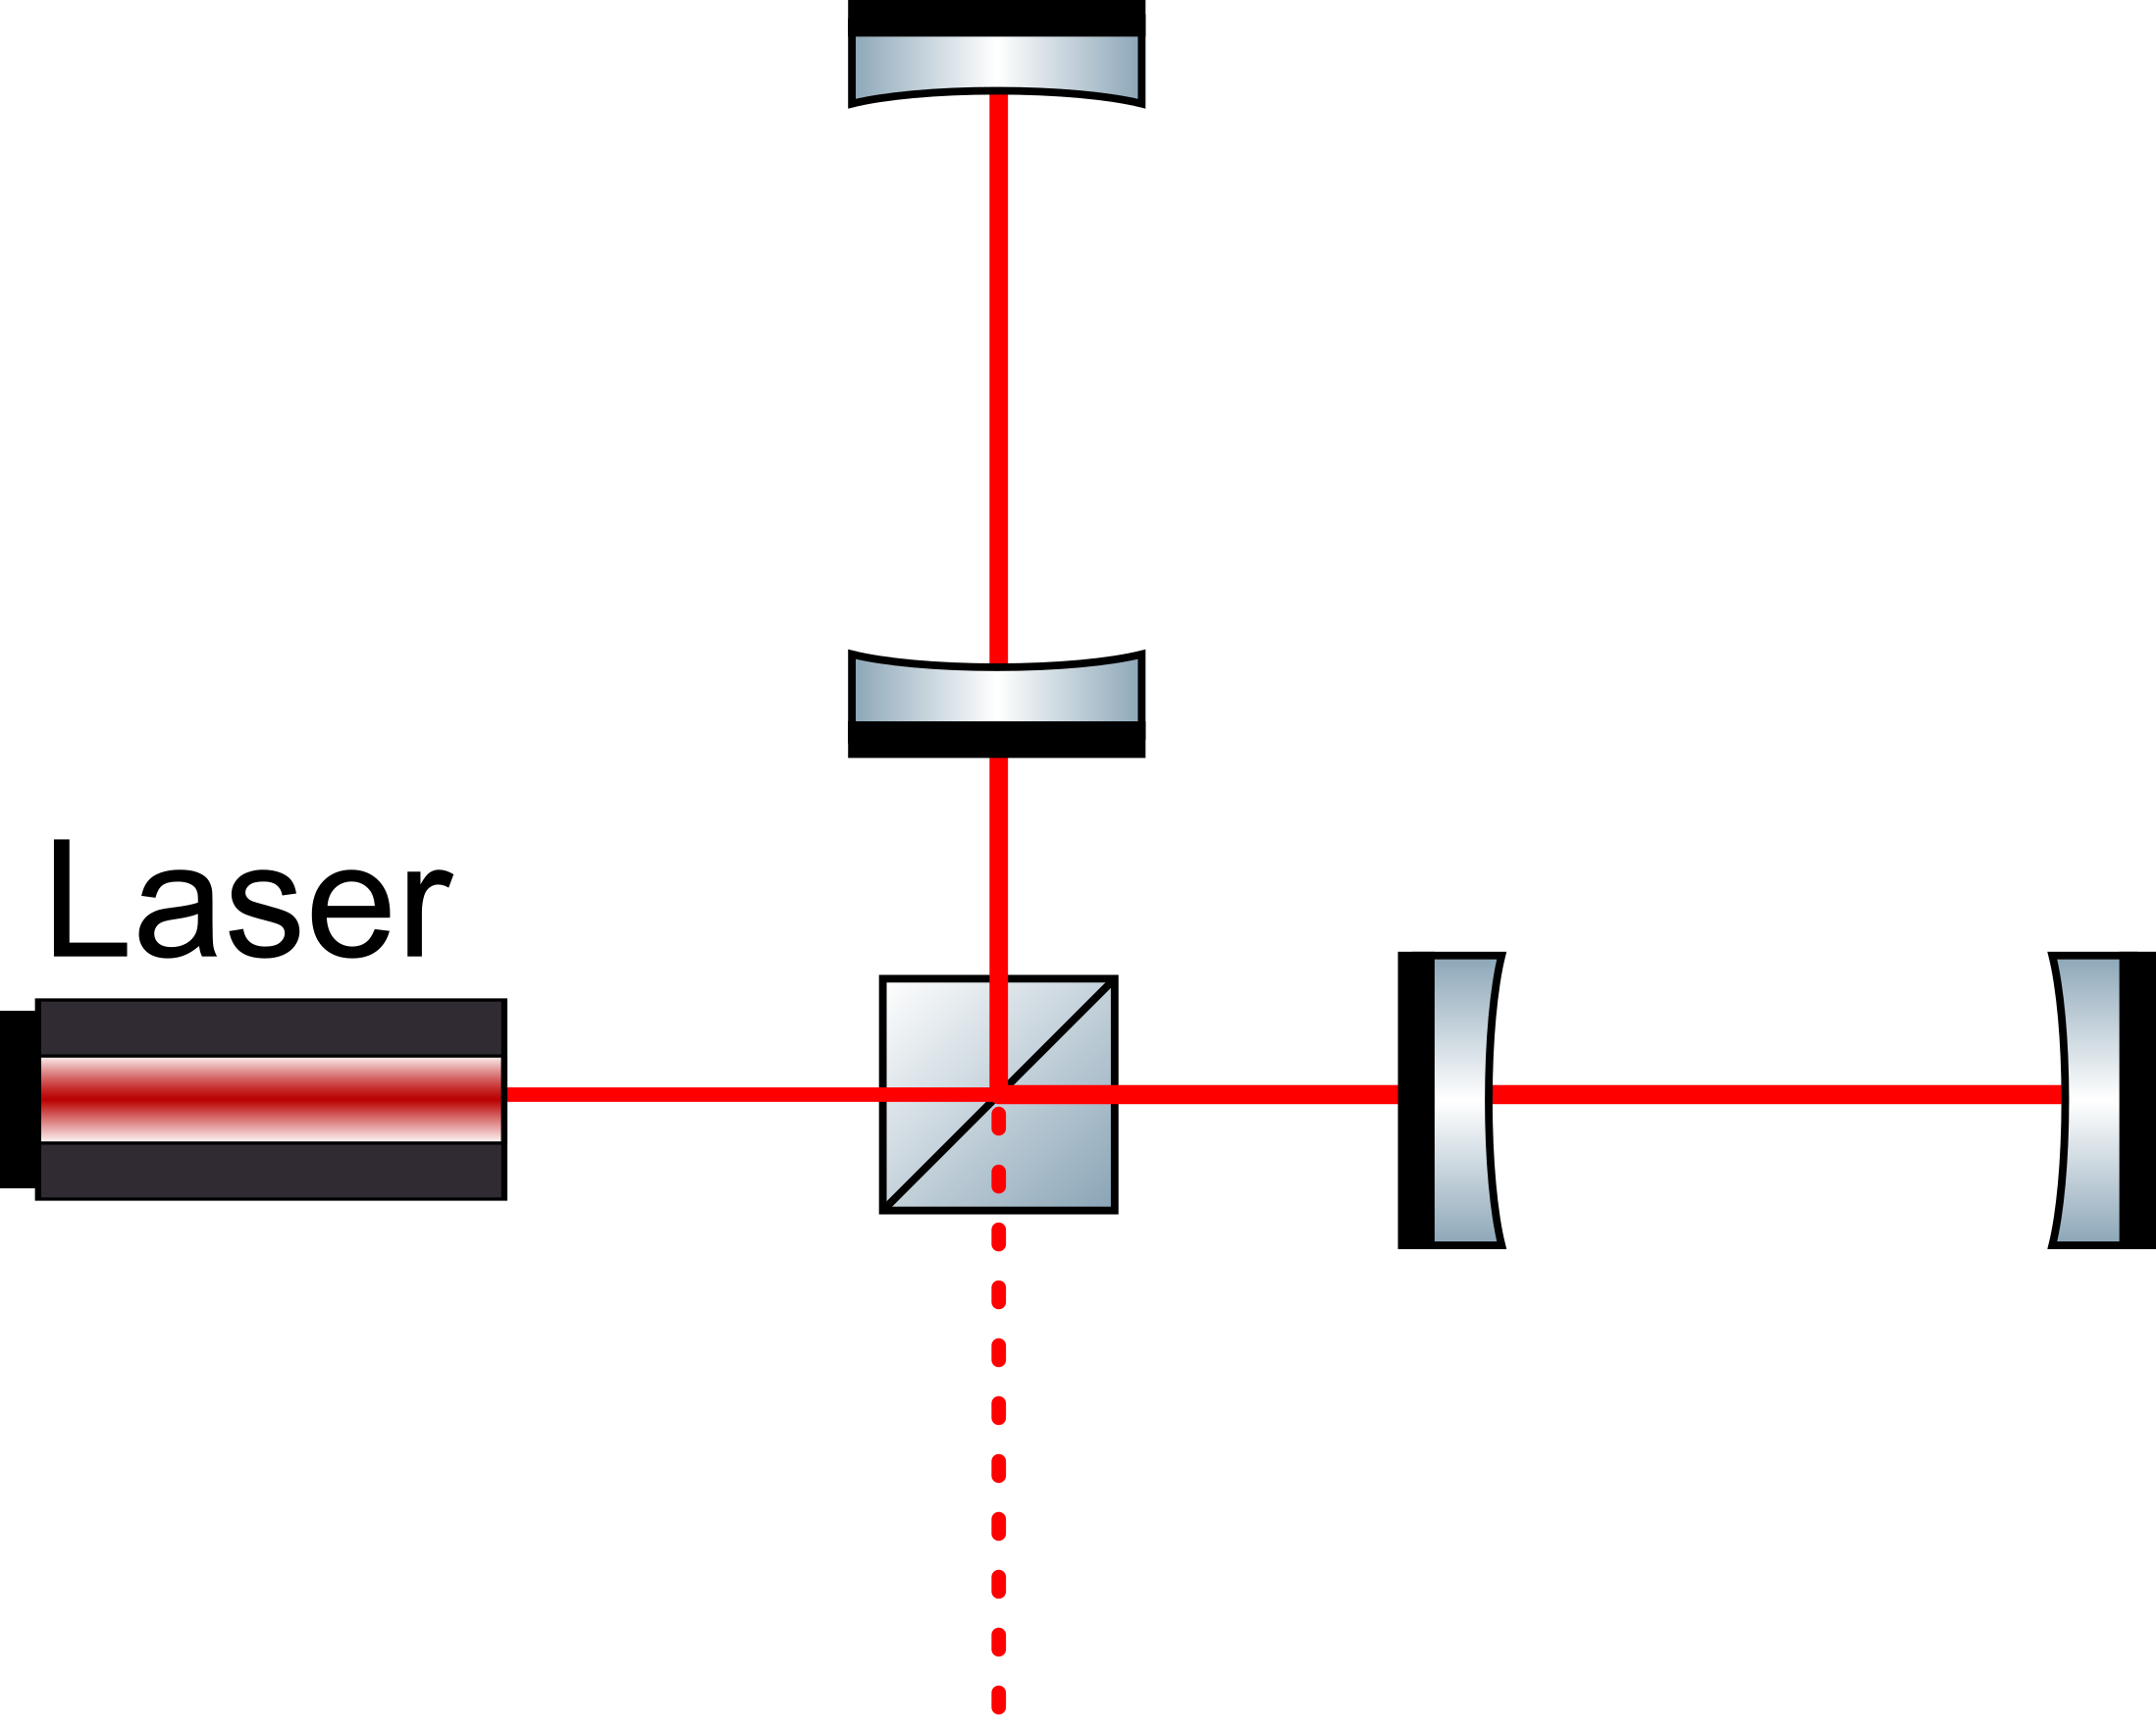
\includegraphics[width=\textwidth]{../Figures/FP_Mich.png}
				\caption{Fabry Perot Michelson}
				\label{fig:FPMich}
			\end{subfigure}
			\hfill
			\begin{subfigure}[b]{0.3\textwidth}
				\centering
				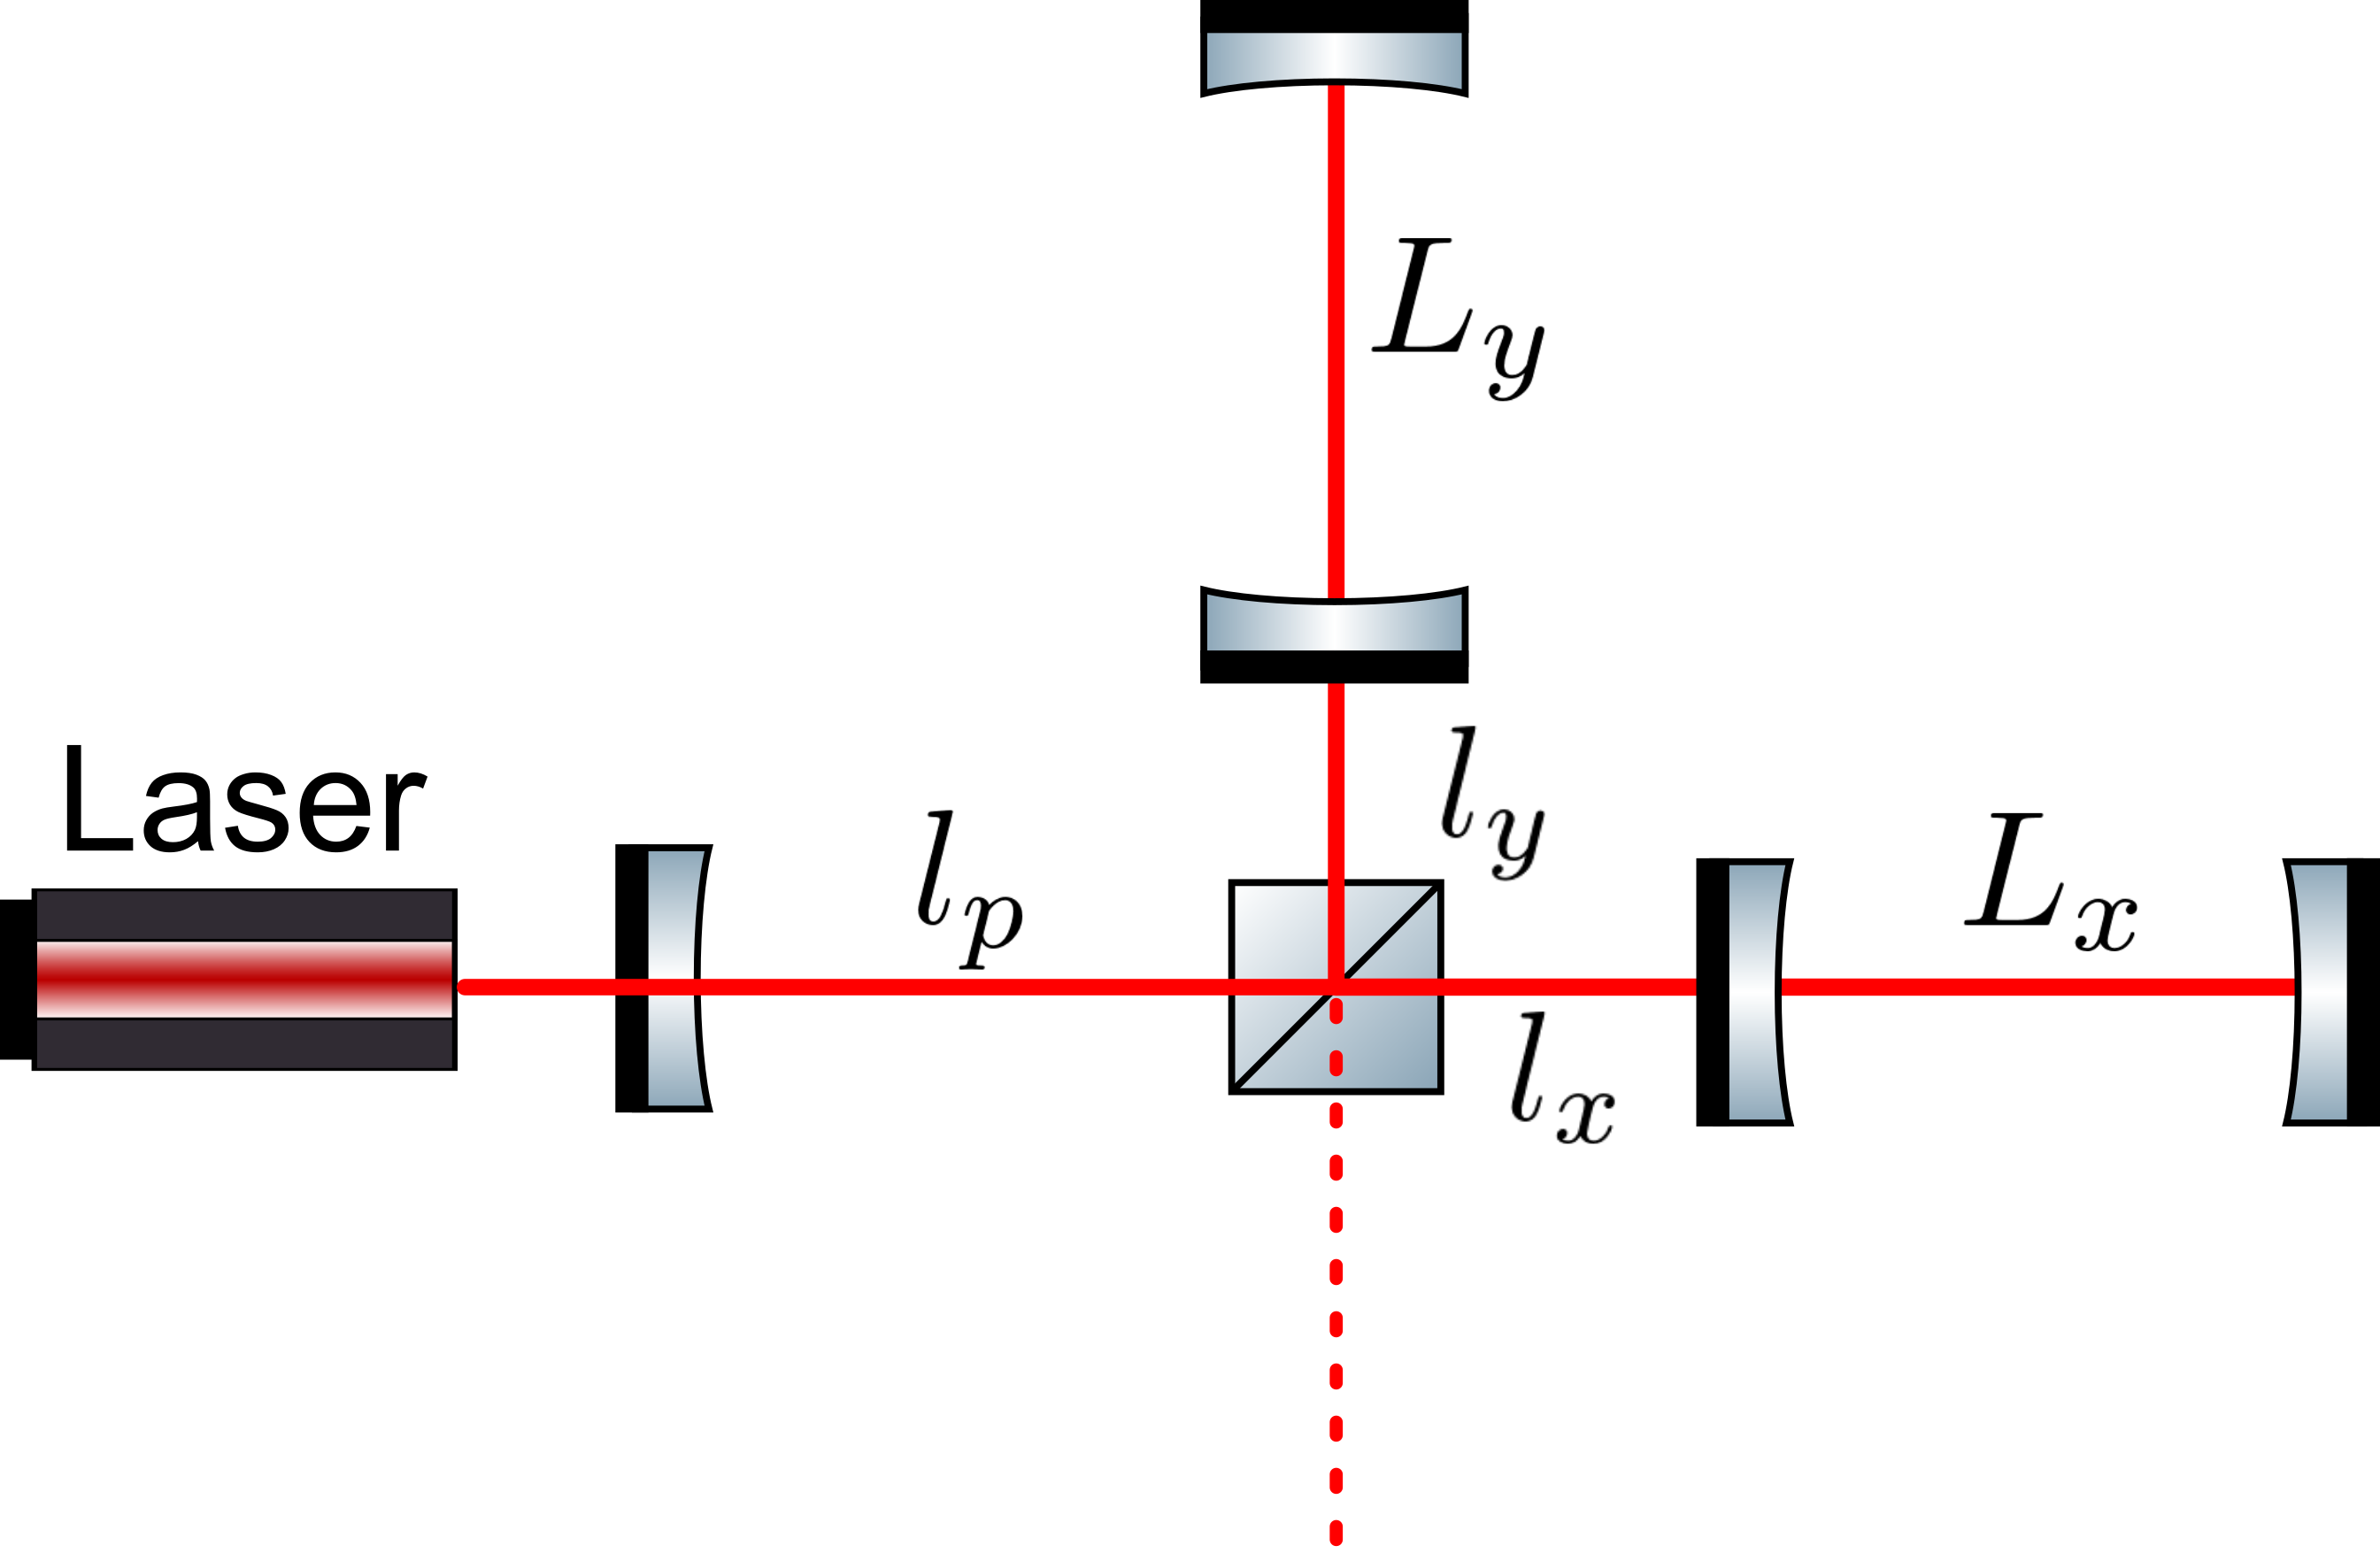
\includegraphics[width=\textwidth]{../Figures/PRFP_Mich.png}
				\caption{Power Recycled Fabry Perot}
				\label{fig:PRFPMich}
			\end{subfigure}
			\hfill
			\begin{subfigure}[b]{0.3\textwidth}
				\centering
				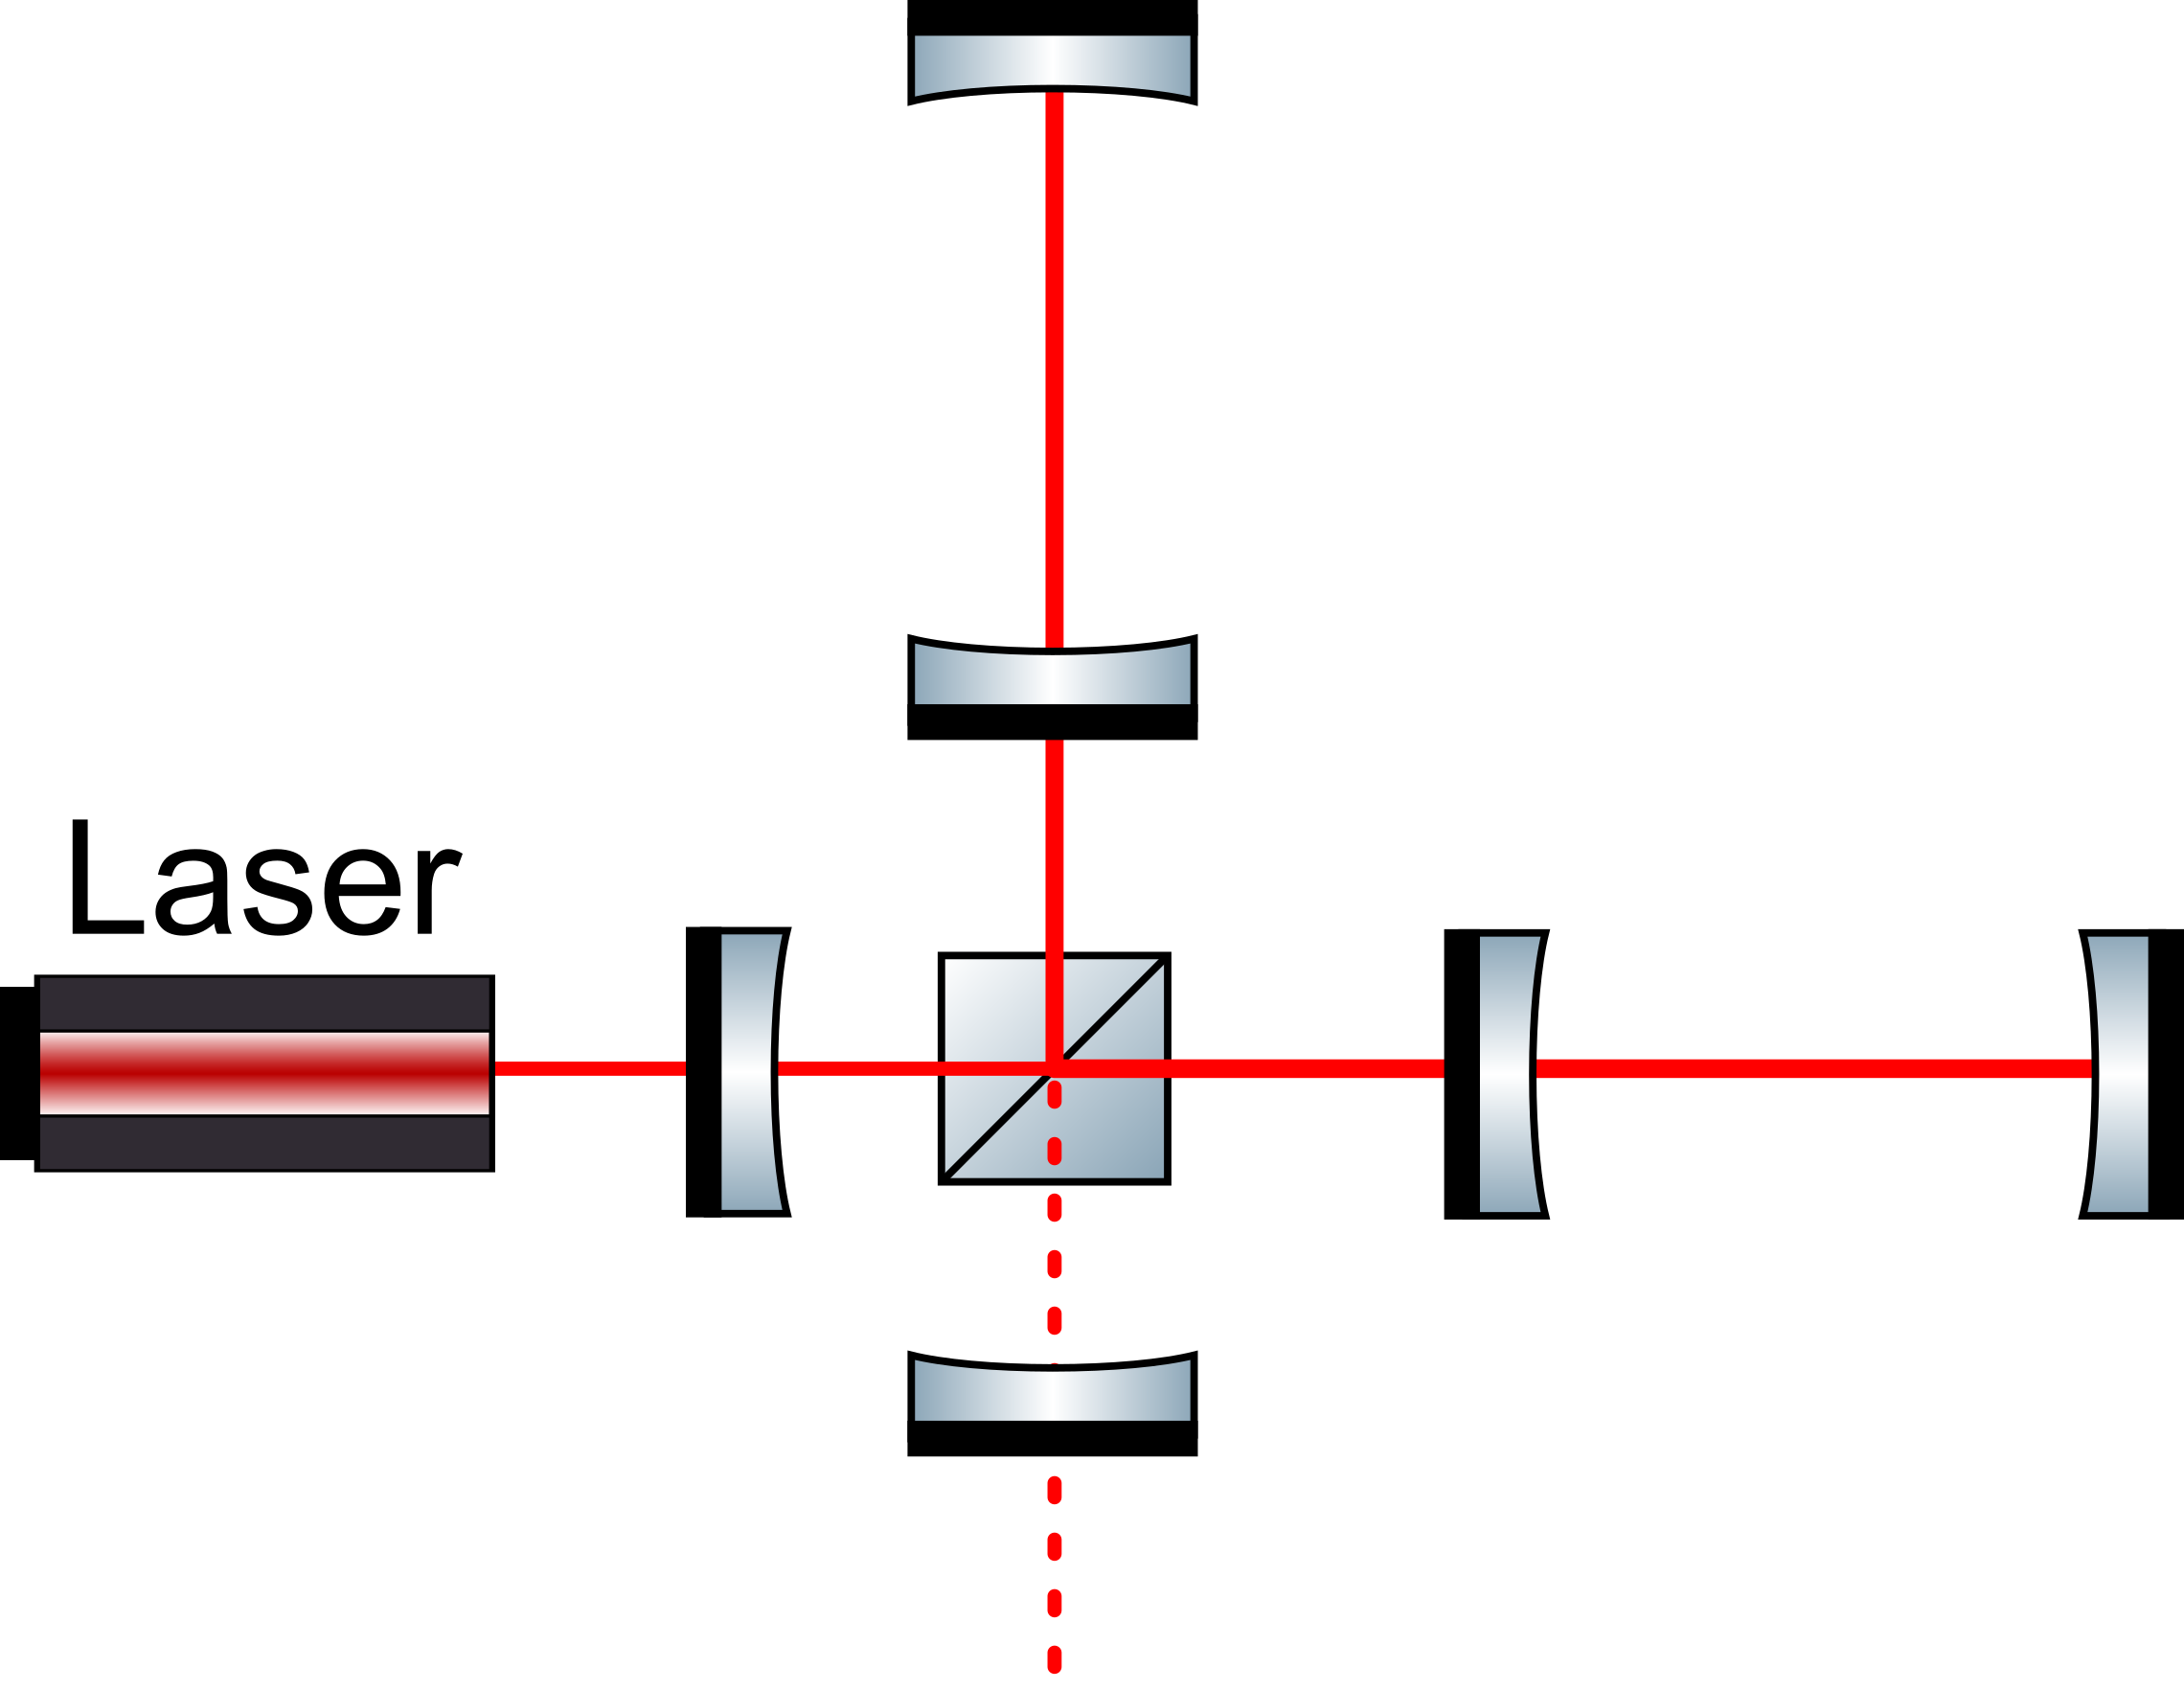
\includegraphics[width=\textwidth]{../Figures/DRFP_Mich.png}
				\caption{Dual Recycled Fabry-Perot}
				\label{fig:DRFPMich}
			\end{subfigure}
			\caption{Interferometer configurations}
			\label{fig:three graphs}
		\end{figure}

		If the interferometer is operating such that the intensity at the antisymmetric port is close to null, conservation of energy requires that the power from the arms will reflect back towards the input laser.  Fritschel et al [\cite{Fritschel_Readout} \cite{FritschelLightRecycling}] shows the effect of adding a partially reflecting mirror to increase the optical gain of the Michaelson for the sidebands and carrier fields.
		
		Section \ref{FPmich} showed that the Michelson interferometer with Fabry Perot arms can be represented by a single cavity response.  Therefore it is useful to model a power recycled interferometer by using a coupled cavity approach shown in Figure[PowerFPsimple] where the end mirror is replaced with the reflected field of the Michelson on a bright fringe.  Here the reflectivity and transitivity of the power recycling mirror (PRM) is denoted by $r_p$ and $t_p$, respectively.  
		
		In this configuration, the effective length of the cavity is
		the average path between the power recycling mirror and the high reflectivity surfaces of the input test masses,
		\begin{equation}
		l_{\text{PRC}} = l_\text{p} + \frac{l_x + l_y}{2}
		\end{equation}
		The circulating power in the cavity is given by equation \ref{c_FP} but uses the reflectivity of arm cavities,
		\begin{equation}
		E_{\text{PRC}} = \frac{t_p}{1- r_p r_{\text{FPM}}   e^{-2ik l_{\text{PRC}}}}E_{\text{in}}
		\end{equation}
		where $r_{\text{FPM}}\approx 1 - \frac{\mathbb{F}}{\pi} L_{\text{rt}} $ for high finesse cavities, which is a valid approximation for the advanced LIGO arm cavities since their values for finesse can be around 250 or higher depending on the losses.  This means the circulating power in the recycling cavity while on resonance can be expressed by
		\begin{equation}
		P_{\text{PRC}} = \frac{1-r_p^2}{\bigg[ 1 - r_p  (1 - \frac{\mathbb{F}}{\pi} L_{\text{rt}})   \bigg]^2}P_{\text{in}}
		\end{equation} 
		By taking the derivative with respect to the reflectivity of PRM and setting to zero, the optimal power recycling tuning is linearly proportional to the round trip loss,
		\begin{equation}
		r_{\text{opt}}  = 1 - \frac{\mathbb{F}}{\pi} L_{\text{rt}}
		\end{equation}
		so it important to keep the arm cavity losses as low as possible and this also limits the ability to increase the finesse.
		
		Adding a power recycling mirror will be equivalent to introducing higher power into the arm cavities but it will not shape the gravitational wave sideband frequency dependence in any other way.  This can be reasoned qualitatively by imagining the signal sidebands that get created in the arm cavities and propagate to the beam splitter where they will combine, however, the stretching and squeezing from the gravitational wave pattern will make the x-arm amplitude negative relative to the y-arm.  This makes the anti-symmetric port transmissive to the signal sidebands but the carrier field which mostly gets reflected to the symmetric port will see the power recycling amplification.  This means the beat note between the static carrier field and gravitational wave signal for a power recycled Fabry-Perot interferometer is
		\begin{equation}
		S_{\text{PRFP}} \propto E_0^2 \; \frac{8\pi L}{\lambda} \sqrt{g_{\text{PRC}}} \bigg[\frac{t_1}{1-r_1r_2}\bigg]^2 \bigg[\frac{1}{1 - i \frac{\omega_{\text{\tiny GW}}}{\omega_p}}\bigg] \sin{(k\delta l)} \sin{(\phi_{D})} h_{\text{\tiny GW}}
		\end{equation}
		where $g_{\text{PRC}} = P_{\text{PRC}}/P_{\text{in}}$ is the power recycling gain.
		
		\subsection{Dual-Recycled Fabry-Perot Interferometers}\label{DRMI}
		
		One of the biggest changes made between initial and advanced LIGO was the addition of a signal recycling mirror at the antisymmetric port (Figure [DRFPMI]). In the previous section, it was shown that the gravitational wave sensitivity was improved by adding a power recycling cavity to increase the effective input power into the Fabry-Perot cavities.  Adding another partially reflecting optic called the signal recycling mirror (SRM) at the antisymmetric port to create a resonant cavity will shape the interferometer's response to gravitational waves.  This allows for some flexibility in optimizing the instrument for specific sources such as binary neutron stars, but it also creates a more broadband response at higher frequencies while allowing the arm cavity finesse and/or power recycling to impart more power.
		
		\begin{figure}[h]
			\centering
			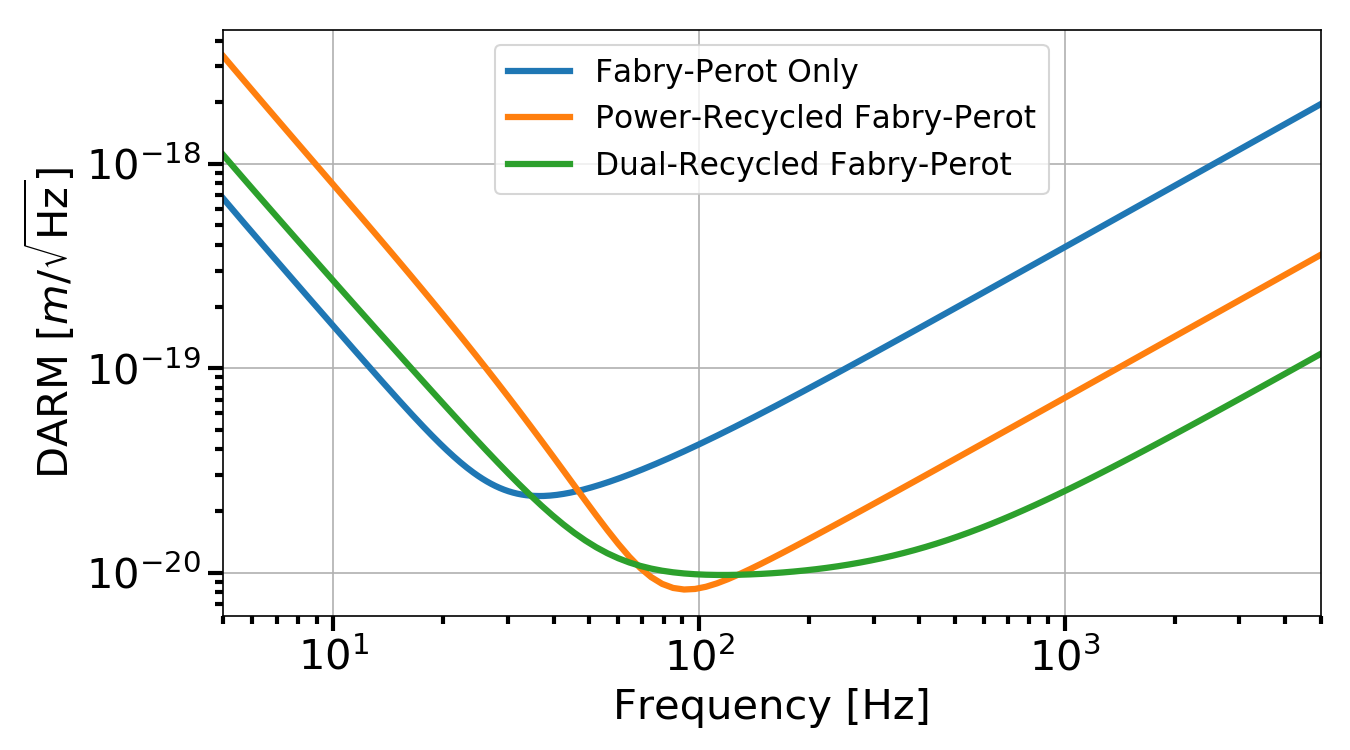
\includegraphics[width=1.0 \textwidth]{../Figures/QM_Limited_Sense.png}
			\caption{Quantum limited sensitivity by combining shot noise and radiation pressure}
			\label{fig:DRMICH_sense}
		\end{figure}
		
		A nice way to model the effect of signal recycling on the gravitational wave sidebands is to combine the SRM and  arm cavity input test mass to create a combined  mirror that is dependent on the round trip phase, $\phi_s$ of the signal recycling cavity.  The SRM will have a reflectivity and transmissivity equal to $r_s$ and $t_s$, respectively, so the combined mirror will have a reflectivity and transmissivity equal to
		\begin{equation}
		r_{1+s} = \frac{r_1 - r_s e^{-2i\phi_s}}{1- r_1 r_s e^{-2i\phi_s}}
		\end{equation}
		\begin{equation}
		t_{1+s} = \frac{t_1 t_s e^{i\phi_s}}{1- r_1 r_s e^{-2i\phi_s}}
		\end{equation}
		where $\phi_s = k \big( l_\text{s} + \frac{l_x + l_y}{2} \big)	$ is the average signal recycling length.
		Plugging this into equation \ref{Egw} in place of the input test mass reflectivity shows that the cavity pole is directly affected by the signal recycling properties, namely, the SRM reflectivity and the microscopic detuning of the length. The field propagating to the true antisymmetric port is in transmission of the signal recycling cavity which is accounted for with the last bracketed term. 
		\begin{equation}
		\begin{aligned}
		E_{\text{AS}}(\pm \omega_{\text{\tiny GW}}) & =  \bigg[ \frac{t_1^2}{1-r_1 r_2}\bigg]  \frac{E_0}{\sqrt{2}} \bigg[\frac{ 1}{1 \pm r_{1+s} r_2 e^{-2i  \omega_{\text{\tiny GW}}  \frac{L}{c}}} \bigg] \bigg[\frac{t_1 t_s e^{i\phi_s}}{1- r_1 r_s e^{-2i\phi_s}}\bigg] ik\Delta L\\
		& \propto \bigg[ \frac{ \text{Constant}}{1 \pm 2 i \frac{r_{1+s} r_2}{1- r_{1+s} r_2}  \omega_{\text{\tiny GW}}  \frac{L}{c}}  \bigg]\\
		& \propto \bigg[\frac{\text{Constant}}{1 \pm i \omega_{\text{\tiny GW}}/\omega_{\text{DR}}}\bigg]
		\end{aligned}
		\end{equation}
		Here, the frequency dependence of the differential cavity pole with dual recycling is denoted by
		\begin{equation}
		\begin{aligned}
			\omega_{\text{DR}} 	&=	\frac{1-r_{1+s}r_2}{r_{1+s}r_2}\frac{c}{2L}\\
								&=	\frac{1- r_1r_s e^{-2i\phi_s} }{ (r_1 - r_s e^{-2i\phi_s})r_2} - 1
		\end{aligned}
		\end{equation}
		
		Figure[ifoconfigs]
		The carrier field will also see a gain from the signal recycling cavity equal to
		\begin{equation}
		\sqrt{g_{\text{SRC}}} = \frac{t_s}{1+ r_s r_{\text{FPM}}   e^{-2i\phi_s}}
		\end{equation}
		It is clear from the equations above that the gravitational wave sideband and carrier fields will see the signal recycling cavity effects differently and the responses are highly sensitive to the length detuning of $\phi_s$.
		Putting all the pieces together to get the dual recycled Fabry-Perot interferometer response to gravitational waves,
		\begin{equation}
		S_{\text{DRFP}} \propto E_0^2 \; \frac{8\pi L}{\lambda} \sqrt{g_{\text{PRC}}}\;\sqrt{g_{\text{SRC}}}\; g_{\text{ARM}} \bigg[\frac{1}{1 - i \frac{\omega_{\text{\tiny GW}}}{\omega_{\text{DR}}}}\bigg] \sin{(k\delta l)} \sin{(\phi_{D})} h_{\text{\tiny GW}}
		\end{equation}

		

		The previous sections only considered the effect of Fabry-Perot cavities and recycling mirrors at the antisymmetric port due to a differential length change at the 4 kilometer arms but the Advanced LIGO interferometer has a few different degrees of a freedom which are actively controlled.  This means the signals sampling various ports will have contributions from one or more degrees of freedom.  A good reference for what is expected at the important ports such  as REFL, AS, and POP can be found in \cite{kiwamu_freq1} \cite{kiwamu_freq2} \cite{kiwamu_freq3}
		\subsection{Fundamental Noise Sources}\label{funnoise}
		The proceeding sections describe ways to increase the response of LIGO to gravitational waves; equally as important is the science of characterizing and reducing the noise contributions from everything else.
		
		Noise budget:
		
		\subsubsection{Quantum Noise}

		One fundamental noise source that is limiting LIGO's sensitivity comes from the fluctuations of quantum vacuum entering the anti-symmetric port and coupling to the input laser. A quantum mechanical description of an interferometer was constructed by Caves \cite{CavesQMNoise}\cite{Caves2photon} \cite{CavesOscillator}, where he used electric field operators to show that vacuum fluctuations are the cause of radiation pressure and shot noise in an interferometer.
		
		\textbf{Quantum states}:
		It is well known in physics \cite{Shankar} \cite{Griffiths} that a solution to the quantum harmonic oscillator in the energy eigenbasis employs the annihilation and creation  operators, $\hat{a}^{\dagger}$ and $\hat{a}$, to factorize the Hamiltonian
		\begin{equation}
		\hat{H} = \hbar w (\hat{N} + 1/2)
		\end{equation} 
		where $\hat{N} = \hat{a}^{\dagger}  \hat{a}$ is the number operator.  When using this formalism to create a coherent electromagnetic field, it is useful to define a unitary operator that displaces the vacuum state \cite{GerryKnight}:
		\begin{equation}
		\hat{D} \equiv \hat{D}(\alpha) \equiv \text{exp}(\alpha \hat{a}^{\dagger} - \alpha^{*} \hat{a} ) = e^{-\frac{\vert{\alpha}\vert^2}{2}} e^{\alpha \hat{a}^{\dagger} } e^{\alpha^{*} \hat{a} }
		\end{equation}
		$\hat{D}(\alpha) = \hat{D}^{-1}(\alpha) = \hat{D}(-\alpha)$
		\begin{equation}
		\begin{aligned}
		\hat{D}^\dagger&\, \hat{a} 		\,\hat{D}			= \hat{a} + \alpha \\ 
		\hat{D}^\dagger&\, \hat{a}^\dagger \,\hat{D} 		= \hat{a}^\dagger + \alpha^*
		\end{aligned}
		\end{equation}
		\begin{equation}
		\ket{\alpha} = \hat{D} \ket{0} =  e^{-\frac{\vert{\alpha}\vert^2}{2}} e^{\alpha \hat{a}^{\dagger} } \ket{0}
		\end{equation}
		
		
		\textbf{Radiation Pressure}
		
		One might naively think that power fluctuations in the laser cause radiation pressure effects on the test masses which will result in noise.  However, if the 50/50 beamsplitter is perfect, then the momentum transfer to each test mass will be a common length change and will not vary the intensity at the antisymmetric port (or the symmetric port for that matter).
		
		The concept of quantum radiation pressure arises from considering plane wave waves entering the interferometer from both the symmetric and anti-symmetric ports.  This method is similar to the input-output methods of section \ref{michelson}, however, the difference being that the beamsplitter will couple the electric fields from the input laser and quantum vacuum.
		
		To start, consider the electric fields combining at the beamsplitter from both ports to strike the mirrors, respectively,
		\begin{subequations}\label{exey}
		\begin{equation}
		E_x = \frac{1}{\sqrt{2}} \bigg[ iE_0 +   E_{AS,in} \bigg]
		\end{equation}
		\begin{equation}
		E_y = \frac{1}{\sqrt{2}} \bigg[  E_0 + i E_{AS,in} \bigg]
		\end{equation}
		\end{subequations}
		The intensities hitting each test mass will be
		\begin{subequations}
		\begin{equation}
		\vert E_x \vert^2 = \frac{1}{2} \bigg[ \vert E_0 \vert^2 + \vert E_{AS,in} \vert^2  + i(E_0 E^*_{AS,in} - E_0^*E_{AS,in} )\bigg]
		\end{equation}
		\begin{equation}
		\vert E_y \vert^2 = \frac{1}{2} \bigg[ \vert E_0 \vert^2 + \vert E_{AS,in} \vert^2  - i(E_0 E^*_{AS,in} - E_0^*E_{AS,in} )\bigg]`
		\end{equation}
		\end{subequations}
		
		The differential momentum transfer between the two masses will be equal to the differences in intensities:
		\begin{equation}\label{momentumtranfer}
		\begin{aligned}
		 \mathbf{P} 	&= \frac{2 \hbar \omega}{c} \bigg( \vert E_x \vert^2 - \vert E_y \vert^2 \bigg) \\
						&= \frac{2 \hbar \omega}{c} \bigg( E_0 E^*_{AS,in} - E_0^*E_{AS,in} \bigg)\\
		\Rightarrow	\mathbf{\hat{P}}&= \frac{2 \hbar \omega}{c} \bigg( \hat{a}_1^{\dagger} \hat{a}_2 - \hat{a}_2^{\dagger} \hat{a}_1 \bigg)
		\end{aligned}
		\end{equation}
		The last part of equation \ref{momentumtranfer} replaces the classical electric fields with creation and annihilation operators for the symmetric input mode ($\hat{a}_1^{\dagger}$, $\hat{a}_1$) and antisymmetric input mode ($\hat{a}_2^{\dagger}$, $\hat{a}_2$) modes. Recall that there is a well established convention denoting the wave function of the two dimensional modes of the quantum harmonic oscillator \cite{GerryKnight}, $\ket{\alpha,\beta}$, where $\alpha$ denotes the input symmetric mode and $\beta$ refers to the input antisymmetric mode.
		\begin{equation}
		\ket{\alpha,0} = \hat{D}_1(\alpha) \ket{0,0}
		\end{equation}
		The interesting results arising from this formulation is the expectation value
		\begin{equation}
		\langle \mathbf{\hat{P}} \rangle = \bra{\alpha,0} \mathbf{\hat{P}}\ket{\alpha,0} = 0
		\end{equation}
		And the variance 
		\begin{equation} 
		\begin{aligned}
		\Delta \mathbf{P}^2 &= \langle \mathbf{\hat{P}}^2 \rangle  - \langle \mathbf{\hat{P}} \rangle^2 \\
							&= \bigg(\frac{2 \hbar \omega}{c}\bigg)^2 \bra{\alpha,0}  \hat{a}_1^{\dagger}  \hat{a}_2  \hat{a}_1  \hat{a}_2^{\dagger} + \hat{a}_2^{\dagger}  \hat{a}_1  \hat{a}_2  \hat{a}_1^{\dagger}
							- \hat{a}_2^{\dagger}  \hat{a}_1  \hat{a}_1  \hat{a}_2^{\dagger} - \hat{a}_1^{\dagger}  \hat{a}_2  \hat{a}_2  \hat{a}_1^{\dagger} \ket{\alpha,0}\\
							&= \bigg(\frac{2 \hbar \omega}{c}\bigg)^2 \vert \alpha \vert^2
		\end{aligned}
		\end{equation}
		For some time interval, input laser power consisting of $\langle N \rangle =\vert\alpha \vert^2$ photons for a time interval $\Delta T$ is,
		\begin{equation}
		P_{in} = \frac{\hbar \omega}{\Delta T} \vert \alpha \vert^2
		\end{equation}
		To solve for the amplitude spectral density of the displacement, Newton's second law can be applied in the frequency domain
		\begin{equation}
		M (2\pi f)^2 \tilde{x}(f) = \tilde{F}(f) = \frac{\Delta \mathbf{P}}{\Delta T}
		\end{equation}
		The force spectrum is white because the impacting photons arrive randomly.
		
		Solving for the displacement,
		\begin{equation}
		\tilde{x}_{RP}(f) = \sqrt{\frac{\hbar \omega}{\Delta T} P_{in}} \frac{1}{2Mc (\pi f)^2}
		\end{equation}
	
		The noise spectral density for $M=40kg$, $P_{in}=125$W, and $\lambda=1064$nm
		\begin{equation}
		\tilde{h}_{RP}(f) = 2.04\times 10^{-20} \frac{1}{f^2} \; \bigg[ \frac{\text{Strain}}{\sqrt{\text{Hz}}}\bigg]
		\end{equation}
		\textbf{Shot Noise}
		Another way that quantum fluctuations can vary the antisymmetric port output is by adding phase noise.  Imagine holding the test masses rigidly such that the only effects on the output light is due to a phase change in the laser light in the arms. By using the same formulation for radiation pressure but propagating the fields back to the beam splitter, equations \ref{exey} will have extra phase,
		
		\begin{subequations}\label{exeyout}
		\begin{equation}
		E_{x,out} = \frac{1}{\sqrt{2}} \bigg[ iE_0 +   E_{AS,in} \bigg] e^{-i2kL_x}
		\end{equation}
		\begin{equation}
		E_{y,out} = \frac{1}{\sqrt{2}} \bigg[  E_0 + i E_{AS,in} \bigg] e^{-i2kL_y}
		\end{equation}
		\end{subequations}
		
		Antisymmetric port output electric field is
		\begin{equation}
		\begin{aligned}
		E_{AS,out} 	&= \frac{1}{\sqrt{2}} (E_{x,out} + iE_{y,out})\\
					&= i e^{-ikL_x-ikL_y} \big[\cos(\Delta \phi) E_0 - \sin(\Delta \phi) E_{AS,in}\big]
		\end{aligned}
		\end{equation}
		where $\Delta \phi = k(L_x-Ly)$
		Output intensity,
		\begin{equation}
		\begin{aligned}
		\mathbf{I}_{AS,out} 		&= \vert E_{AS,out}\vert^2 \\
									&= \bigg[ \cos^2(\Delta \phi)\vert E_0\vert^2 + \sin^2(\Delta\phi)\vert E_{AS,in}\vert^2 - \sin(\Delta\phi)\cos(\Delta\phi) \big[E_0 E^*_{AS,in} + E_0^* E_{AS,in}\big] \bigg]\\
		\Rightarrow	
		\hat{\mathbf{I}}_{AS,out} 	&= \bigg[ \cos^2(\Delta \phi)a_1^{\dagger}a_1 + \sin^2(\Delta\phi)a_2^{\dagger}a_2 - \sin(\Delta\phi)\cos(\Delta \phi) \big[a_1^{\dagger}a_2 + a_2^{\dagger}a_1 \big] \bigg]\\	
		\end{aligned}
		\end{equation}
		
		The expectation value for the intensity using an input coherent laser with $\alpha$ and quantum vacuum input at the antisymmetric port is
		
		\begin{equation}
		\begin{aligned}
		\langle \hat{\mathbf{I}} \rangle 	&= \bra{\alpha,0} \hat{\mathbf{I}}_{AS,out} \ket{\alpha,0}\\
							&= \cos^2(\Delta \phi) \vert \alpha \vert^2
		\end{aligned}
		\end{equation}
		
		which matches the classical description of a Michelson output.
		
		Following the same methods to calculate the radiation pressure, photon number variance is 
		\begin{equation} 
		\begin{aligned}
		\Delta \mathbf{I} 	&= \sqrt{\langle \mathbf{\hat{I}}^2 \rangle  - \langle \mathbf{\hat{I}} \rangle^2)} \\
							&= \vert \alpha \vert \big[ \cos^2(\Delta \phi)\ \big] 
		\end{aligned}
		\end{equation}
		
		\begin{equation}
		I = N \cos^2(\Delta \phi)
		\end{equation}
		
		\begin{equation}
		\frac{\partial I}{\partial \phi} = - 2 \vert \alpha \vert^2\cos(\Delta \phi) \sin(\Delta \phi)
		\end{equation}
		
		\begin{equation}
		\delta \phi = \sqrt{\frac{\hbar \omega}{ P_{in}}} \cot(\Delta \phi)
		\end{equation}
		Here $\delta \phi$ is the microscopic change in phase due to shot noise, whereas $\Delta\phi$ is the DC offset in the arm lengths to begin with. So in general, the shot noise contribution is dependent on the amount of light present at the anti-symmetric port and this will vary depending on what type of read out that is implemented.
		
		\begin{equation}
		\tilde{h}_{SN}(f) = 8.2\times 10^{-22} \; \bigg[ \frac{\text{Strain}}{\sqrt{\text{Hz}}}\bigg]
		\end{equation}
		Unsurprisingly, the variance is proportional to the amount of photons present and the phase difference between the interferometer arms.
		Interestingly, there are a few subtleties associated with measuring the noise, it is assumed here that the interferometer readout is a simple photodetector located at the antisymmetric port.  However,it is possible to measure the light at two different phases (90 degrees apart) and subtract the results.   Also, in section \ref{michelson}, there is a freedom to choose the readout scheme of the interferometer (heterodyne or homodyne) which will also affect the overall quantum noise.
		
		\subsubsection{Seismic Noise}
		Reference:[Kissel Thesis]
		Seismic noise will be the low frequency barrier for all terrestrial gravitational-wave detectors.  The main contributions to seismic noise are primarily caused by either natural occurrences  (tectonic plates, wind driven microcosms, oceanic storms etc) or man-made disturbances (heavy automotive traffic, industrial machinery, etc) which contribute to the background hum of motion.       By using seismic isolation platforms and quadruple suspensions, the noise contribution can be attenuated for frequencies larger than ~1Hz; this is a tremendous upgrade from the mostly passive isolation methods used in initial LIGO.
		
		Compare low and high noise microseisms
		\cite{BlairBook}
		The Advanced LIGO's solution to the low frequency wall is comprised of seismic isolation platforms and multi-level suspensions.
		
		\cite{driggers_global}
		
		\cite{fabrice_sei1}
		
		\cite{fabrice_sei2}
		
		\cite{fabrice_strat}
		
		\cite{sei_isol}
		
		\cite{Hang_LF}
		
		\cite{Fritschel_alignment}
		
		\subsubsection{Thermal Noise}
		Brownian motion \cite{brownian_einstein} is the random movement of particles suspended in a fluid.  The LIGO test masses, which make up the 4 kilometer long Fabry Perot cavities, are a large macroscopic object but their constituent atoms are excited by the ambient temperature and have associated random motion. Those atoms are interconnected and allow for the propagation of an infinite number of elastic wave modes that contain random relative phases and the linear superposition of the modes create distortions that result in thermal noise.	
		
		There are two important points that the Fluctuation-Dissipation theorem is based off:
		
		1) When in thermal equilibrium, a system's response to random fluctuations will be the same as when a small force applied.
		2) When a system dissipates energy, there exists a reverse process that allows energy to flow back into the system.
		
		A good way to start analyzing thermal noise is to consider a simple harmonic oscillator with mass $m$, that is in a thermal bath with a damping force, $F=-b\dot{x}(t)$.
		\begin{equation}
		\ddot{x}(t) + \gamma \dot{x}(t) + \omega_{0}^2 x(t) = F/m
 		\end{equation}
		Here, $\gamma = b/m$ and the force, $F$, can be described by white noise.  In this case, the force represents work being done on the system by the external world whereas the damping factor is the release of the system's energy to the outside world.  By taking the Fourier transform, the equation of motion becomes
		\begin{equation}\label{harmonic}
		\tilde{x}(f) = \frac{\tilde{F}(f)}{m} \; \frac{1}{\omega^2 +i \gamma \omega + \omega_{0}^2} 
		\end{equation}
		This implies that the spectral density for viscous damping is
		\begin{equation}\label{svis}
		S_{Vis} = \frac{S_F}{m^2} \; \frac{1}{(\omega^2 -\omega_{0}^2)^2 + (\gamma\omega)^2}
		\end{equation}
		Because the noise is due to a thermal bath, the integrated power over all frequencies must satisfy this equation
		\begin{equation}
		\frac{1}{2} \int_{-\infty}^{\infty} S_{Vis} (\omega) \frac{\text{d}\omega}{2\pi} = \frac{k_B T}{m\omega_{0}^2}
		\end{equation}
		where $k_B$ is the familiar Boltzmann's constant and $T$ is the ambient temperature.  Solving the integral and plugging the result for $S_F$ back into the equation \ref{svis} gives the power spectrum for viscous damping,
		\begin{equation}\label{vis}
		S_{Vis} = \frac{4k_B T \gamma}{m} \frac{1}{(\omega^2 - \omega_{0}^2)^2 + (\gamma\omega)^2}
		\end{equation}
		This equation shows that for three different frequency regimes, the response can vary wildly.
		\begin{subequations}
			\begin{equation}
			\omega<< \omega_{0} \rightarrow S_{vis} = \frac{4k_B T}{m Q \omega_{0}^3}
			\end{equation}
			\begin{equation}
			\omega \approx \omega_{0} \rightarrow S_{vis} = \frac{4k_B T}{m \omega_{0}^3} Q
			\end{equation}
			\begin{equation}
			\omega >> \omega_{0} \rightarrow S_{vis} = \frac{4k_B T}{m Q} \frac{\omega_0}{\omega^4} 
			\end{equation}
		\end{subequations}
		where $Q=\omega_{0}/\gamma$ is commonly known as the quality factor of a resonator.  Qualitatively, this is directly proportional to the resonance height and its thinness.  Figure [visthermalnoise] shows the resultant frequency dependent power spectrum for a few different quality factors, for higher $Q$ systems the amount of noise contribution from thermal noise is reduced at frequencies above the resonance.  Another commonly used definition of the quality factor is the amount of energy loss per cycle, if the $Q$ of a system is high, then the amount of energy loss per oscillation is very small and will take a longer time returning to equilibrium.  A good description of the quality factor and its application to gravitational wave detectors can be found in section 7.5 of \cite{Saulson}.
		
		As system's mode number increases, the previous analysis becomes very difficult to solve analytically. However, the connection between a damped harmonic oscillator's energy loss and power spectrum can be described generically using the Fluctuation Dissipation Theorem,
		\begin{equation}\label{FD}
		S_x(f) = \frac{k_B T}{\pi^2 f^2} \vert \operatorname{\mathbb{R}e} (Y(f)) \vert
		\end{equation}
		where $Y(f)$ is the complex mechanical admittance (inverse of the impedance) of a system. The physical interpretation of equation \ref{FD} can be viewed as a tunnel of energy between a system of interest and the outside world.  If there is an ability to couple energy from one system to another via some process, then the reverse must be true as well. This subtle but powerful statement can be applied generally.  For example, a resistor which is able to dissipate thermal energy when current is flowing through it will convert random external temperature fluctuations into stray currents that results in $Johnson$ $Noise$.
		
		The mechanical admittance of a system is defined as $Y(f) = \dot{x}(f)/F(f)$, which can be written down directly for a damped harmonic oscillator using equation \ref{harmonic},
		\begin{equation}
			\begin{aligned}
			\frac{\dot{x}(f)}{F} &= \frac{i \omega}{m} \frac{1}{\omega_{0}^2 - \omega^2 +i\gamma \omega}\\
								 &= \frac{i\omega}{m} \frac{(\omega_{0}^2 - \omega^2 - i \gamma \omega)}{(\omega_0^2 - \omega^2)^2 + (\gamma \omega)^2}
			\end{aligned}
		\end{equation}
		and by plugging this into the fluctuation dissipation theorem, the power spectral density matches equation \ref{vis} for the viscous damping.  To extend the usage further, consider the thermal noise from a solid which has some thermoelastic dissipation from an internal mode given by $F_{diss} = -k(1+\phi_L) x(t) $ where the phase term comes from the lag between applied force and the system's response to said force.  By solving Newton's second law with this new damping term, the displacement spectrum becomes 
		\begin{equation}
		\tilde{x}(f) =  \frac{\tilde{F}}{m} \; \frac{1}{(1 + i\phi_L ) \omega_{0}^2 - \omega^2 }
		\end{equation}
		Unlike the previous example of viscous damping, the integral for thermoelastic dissipation only holds for some frequency regime but implementing the fluctuation dissipation theorem leads directly to the noise power spectrum,
		\begin{equation}
			S_{TD}(f) =  \frac{4k_B T \omega_{0}^2 \phi_L}{m \omega} \frac{1}{(\omega^2 - \omega_{0}^2)^2 + (\omega_{0}\phi_L)^2}
		\end{equation}
		The frequency response will also be different compared to viscoelastic dissipation,
		\begin{subequations}
			\begin{equation}
			\omega<< \omega_{0} \rightarrow S_{vis} = \frac{4k_B T}{m Q \omega \omega_{0}^2}
			\end{equation}
			\begin{equation}
			\omega \approx \omega_{0} \rightarrow S_{vis} = \frac{4k_B T}{m \omega_{0}^3} Q
			\end{equation}
			\begin{equation}
			\omega >> \omega_{0} \rightarrow S_{vis} = \frac{4k_B T}{m Q} \frac{\omega_0^2}{\omega^5} 
			\end{equation}
		\end{subequations}
		The structural damping formalism can also be applied to the suspension fibers which hold the 40 kilogram test masses[\cite{SaulsonThermalSus}, \cite{Saulson}] which yield a noise spectral density that contains resonances at a variety of frequencies.  The lower two modes consist of the pendulum and rocking modes, while starting at 500 hertz the violin modes will be seen.  In fact, the violin modes and their harmonics could get rung up from earthquakes and saturate the output mode cleaner's DC photodiodes so the must be actively damped in order to proceed towards nominal low noise.
		
		The largest contribution to the thermal noise for current interferometers do not stem from viscous damping, thermoelastic damping of the substrate, or internal friction of the suspension fibers, but rather from the thermal noise contributed by the dielectric coatings [\cite{HarryThermalCoat}] which cause phase noise at the high reflectivity surface of the mirrors.
		
		
		Thermal Noise [\cite{SaulsonThermalNoise}]
		
		Suspension Thermal Noise \cite{SaulsonThermalSus}
		
		Substrate Thermal Noise [\cite{Saulson}]
		
		Coating Thermal Noise [\cite{HarryThermalCoat}]
		
		Thermal-Optical Noise[\cite{EvansBallmerThermalOptic}]
		
		Residual Viscous damping[\cite{Saulson}]
		
		\subsubsection{Newtonian Noise}
		Although there are some noise sources that can be reduced using increasingly complicated techniques such as various levels of seismic isolation or quantum nondemolition devices as shown above. [\cite{SaulsonNewtonian} and \cite{ThorneNewtonian}].  Newtonian noise caused by fluctuating gravitational fields from the wave motion of the ground is one that cannot easily be reduced but possibly be measured and fed-forward or subtracted off-line.[\cite{DriggersNewtonian}]
		
	
	\section{Squeezed States of Light}

	Virtually all undergraduate quantum mechanics textbooks include a section on the harmonic oscillator [\cite{Shankar}].  An interesting result when solving the Schrodinger equation using creation ($\hat{a^{\dagger}}$) and annihilation $\hat{a}$ operators is the existence of a non-zero energy ground state. 
	
	This effect leads to Quantum Noise, which is a fundamental source that can be improved by modifying the quantum vacuum using correlated photons and injecting the states of light into the antisymmetric port of the interferometer.  Within the LIGO community, this procedure of modifying quantum vacuum is called squeezing. Caves analytically derived the effects of quantum noise on the interferometer as well as the improvement due to	
	
	Losses!?!?!?!?!?!?
	References: [Caves, Dwyer, Kwee, Miao]
	